\documentclass[11pt,oneside,letterpaper]{article}

  % graphicx package, useful for including eps and pdf graphics
  \usepackage{graphicx}
  \usepackage{grffile}
  \usepackage{subfig}
  %\DeclareGraphicsExtensions{.pdf,.png,.jpg}

  % basic packages
  \usepackage{color}
  \usepackage{parskip}
  \usepackage{float}
  \usepackage{microtype}
  \usepackage{url}
  \urlstyle{same}

  \usepackage[hidelinks]{hyperref}
  \hypersetup{colorlinks=true,linkcolor=black,citecolor=black,urlcolor=black}

  \usepackage[]{algorithm2e}

  % reference figures across documents
  % \usepackage{xr}
  % \externaldocument{mers-structure_supp}

  % text layout
  \usepackage{geometry}
  \geometry{textwidth=15cm} % 15.25cm for single-space, 16.25cm for double-space
  \geometry{textheight=22cm} % 22cm for single-space, 22.5cm for double-space

  % helps to keep figures from being orphaned on a page by themselves
  \renewcommand{\topfraction}{0.85}
  \renewcommand{\textfraction}{0.1}

  % bold the 'Figure #' in the caption and separate it with a period
  % Captions will be left justified
  \usepackage[labelfont=bf,labelsep=period,font=small]{caption}
  % \RequirePackage{subfigure}

  % review layout with double-spacing
  %\usepackage{setspace}
  %\doublespacing
  %\captionsetup{labelfont=bf,labelsep=period,font=doublespacing}

  % cite package, to clean up citations in the main text. Do not remove.
  %\usepackage{cite}
  \usepackage{natbib}
  %\renewcommand\citepleft{(}
  %\renewcommand\citepright{)}
  %\renewcommand\citepform[1]{\textsl{#1}}

  \usepackage{amsmath}

  %\usepackage{lineno}
  %\linenumbers

  % Remove brackets from numbering in list of References
  %\renewcommand\refname{\large References}
  %\makeatletter
  %\renewcommand{\@biblabel}[1]{\quad#1.}
  %\makeatother

  \usepackage{authblk}
  \renewcommand\Authands{ \& }
  \renewcommand\Authfont{\normalsize \bf}
  \renewcommand\Affilfont{\small \normalfont}
  \makeatletter
  \renewcommand\AB@affilsepx{, \protect\Affilfont}
  \makeatother

  % comments
  %\usepackage{ulem}
  \definecolor{purple}{rgb}{0.459,0.109,0.538}
  \def\tb#1#2{\sout{#1} \textcolor{purple}{#2}}
  \def\tbc#1{\textcolor{purple}{[#1]}}
  \def\gdc#1{\textcolor{blue}{[#1]}}
  \def\lmc#1{\textcolor{green}{[#1]}}

  % symbols
  % \newcommand{\chiSq}{\chi^{2}_{df}} %LM: ancient DNA? =P %GD: quite :)
  % \newcommand{\dtmrca}{\Delta_\mathrm{TMRCA}}
  % \newcommand{\undtmrca}{\delta_\mathrm{TMRCA}}
  % \newcommand{\dspr}{d_\mathrm{SPR}}

%%% Title & Authors %%%
\title{\vspace{1.0cm} \LARGE \bf Dengue antigenic relationships predict evolutionary dynamics}

  \author[1,2]{Sidney Bell}
  \author[3]{Leah Katzelnick}
  \author[1]{Trevor Bedford}

  \affil[1]{Vaccine and Infectious Disease Division, Fred Hutchinson Cancer Research Center, Seattle, WA, USA}
  \affil[2]{Molecular and Cell Biology Graduate Program, University of Washington, Seattle, WA, USA}
  \affil[3]{Some Department, University of California, Berkeley, CA, USA}

  % \date{\today}

\begin{document}
\maketitle

\begin{abstract}
Dengue virus (DENV), the causative agent of dengue hemorrhagic fever, exists as four genetically distinct serotypes, DENV1-4.
These serotypes are antigenically distinct: symptomatic reinfection with a homotypic virus is very rare, while reinfection with a heterotypic virus is associated with severe disease.
Until recently, it has been assumed that viruses within each serotype are antigenically uniform.
However, specific genotypes within each serotype have been anecdotally associated with varying severity of patient outcomes and epidemic magnitude.
One hypothesis is that each serotype contains overlooked, meaningful antigenic diversity.
While antigenic cartography suggests that heterogeneity may exist within each serotype, its source, extent and impact is unclear.
Here, we analyze a publically available neutralization titer dataset to quantify and phylogenetically characterize the extent of DENV intraserotype antigenic diversity.
We map antigenic changes to specific branches of the virus phylogeny, and interpolate across the tree to estimate the antigenic distance between pairs of viruses based on their relative positions in the phylogeny.
We find that DENV antigenic divergence is tightly coupled to DENV genetic divergence, and is likely a gradual, ongoing process.
We report modest but significant antigenic diversity within each serotype of DENV, and identify a minimum of 12 distinct antigenic clades.
Within each serotype, these antigenic clades are separated by antigenic distances comparable to those associated with differing vaccine efficacy in the recent CYD-TDV vaccine trial.
This suggests that antigenic interactions between specific viral genotypes may contribute to secondary case outcomes and vaccine efficacy.
To understand the impact of this antigenic heterogeneity on real-world DENV population dynamics, we also quantify the extent to which population immunity--accumulated through recent circulation of antigenically similar strains--determines the success and decline of DENV clades in a hyperendemic population.
We find that antigenic fitness is a key determinant of DENV population turnover, although this appears to be driven by coarser serotype-level antigenic differences.
By leveraging both molecular data and real-world population dynamics, these results provide a more nuanced understanding of dengue antigenic evolution, with important ramifications for improving vaccine design and epidemic preparedness.
\end{abstract}

\pagebreak

\section*{Introduction}
Dengue virus (DENV) is a mosquito-borne flavivirus which consists of four genetically distinct clades, canonically thought of as serotypes.
DENV circulates primarily in South America and Southeast Asia, infecting 400 million people annually.
While most of these infections are asymptomatic or mild, $\sim$1--3\% of cases progress to severe dengue hemorrhagic fever, causing approximately 10--15,000 deaths each year.
Unlike most infectious diseases, DENV secondary infections are more likely than primary infections to cause severe disease, with estimates of relative risk of severe dengue of $\sim$24.
Primary infection is usually mild and generates lifelong homotypic immunity and temporary heterotypic immunity, which typically wanes over X--X months.
Subsequent heterotypic secondary infection induces broad cross-protection, and symptomatic tertiary and quaternary cases are very rare.
However, a small subset of secondary infections are enhanced by nonneutralizing, cross-reactive antibodies, resulting in severe disease.
Thus, the antigenic relationships between dengue viruses --- describing whether the immune response generated after primary infection results in protection or enhancement of secondary infection --- are key drivers of DENV case outcomes and epidemic patterns.

While each serotype is clearly genetically and antigenically distinct, it is not clear how sub-serotype clades of DENV interact antigenically.
Each DENV serotype consists of broad genetic diversity, including canonical clades termed `genotypes'.
Specific genotypes have been associated with characteristically mild or severe disease, and heterogeneous neutralization titers suggest that the immune response to some genotypes is more cross-protective than others.
Until recently, it has been assumed that these intraserotype differences are minimally important compared to interserotype differences.
Notably, though, empirical evidence has demonstrated that these genotype-specific differences can drive case outcomes and epidemic severity.
For example, analysis of a longitudinal cohort study demonstrated that specific combinations of primary infection serotype and secondary infection genotype can mediate individual case outcomes.
On a population scale, the DENV1-immune population of Iquitos, Peru, experienced either entirely asymptomatic or very severe epidemic seasons in response to two different genotypes of DENV2.

One explanation for these and similar observations (reviewed in X) is that overlooked intraserotype antigenic variation contributes to these genotype-specific case outcomes and epidemic patterns.
Recent work to antigenically characterize diverse DENV strains suggests that each serotype may contain antigenic heterogeneity, but the source and impact of this heterogeneity is not clear.
Here, we take a phylogenetic approach to characterize the evolutionary basis for observed antigenic heterogeneity among DENV clades.
We also quantify the impact of within- and between-serotype antigenic novelty on real-world DENV population dynamics.

\section*{Results}

% SB general to-do:
% 3 - add references
% 4 - add subfigure labels (A,B, ...)

\subsection{Dengue neutralization titer data}

Antigenic distance between pairs of viruses $i$ and $j$ is experimentally measured using a neutralization titer, which measures how well serum drawn after infection with virus $i$ is able to neutralize virus $j$ in vitro.
To measure the pairwise antigenic distances for a panel of diverse DENV strains, Katzelnick et al. infected naive non-human primates (NHP) with each virus, drew sera at 3 months post-infection, and then titered this sera against a panel of test viruses.
To compare patterns of cross-protection in NHP and humans, they also drew sera from 31 study participants 6 weeks after innoculation with a monovalent component of the NIH dengue vaccine candidate.
This sera was also titered against a broad panel of DENV strains.
As reported by Katzelnick et al., we find generally consistent patterns of neutralization between the NHP and human sera data; see [ref] for a detailed comparison.
In total, our dataset consists of 454 NHP sera titrations spanning the breadth of DENV diversity, and 728 human sera titrations providing deep coverage of a small subset of strains (Figure ~\ref{titered_strains_tree}).

To normalize these measurements, we first take the $log_2$ of each value, such that one titer unit corresponds to one 2-fold drop in neutralization.
We then define antigenic distance between autologous virus-sera pairs (i.e., virus $i$ and serum $i$) as 0.
Normalized titers between $i$ and $j$ are thus calculated as $T_{ij} = log_2(T_{ij}) - log_2(T_{ii})$, such that a higher normalized titer value indicates that serum $i$ is less effective at neutralizing virus $j$, implying greater distance between viruses $i$ and $j$.

\begin{figure}[h]
\begin{centering}
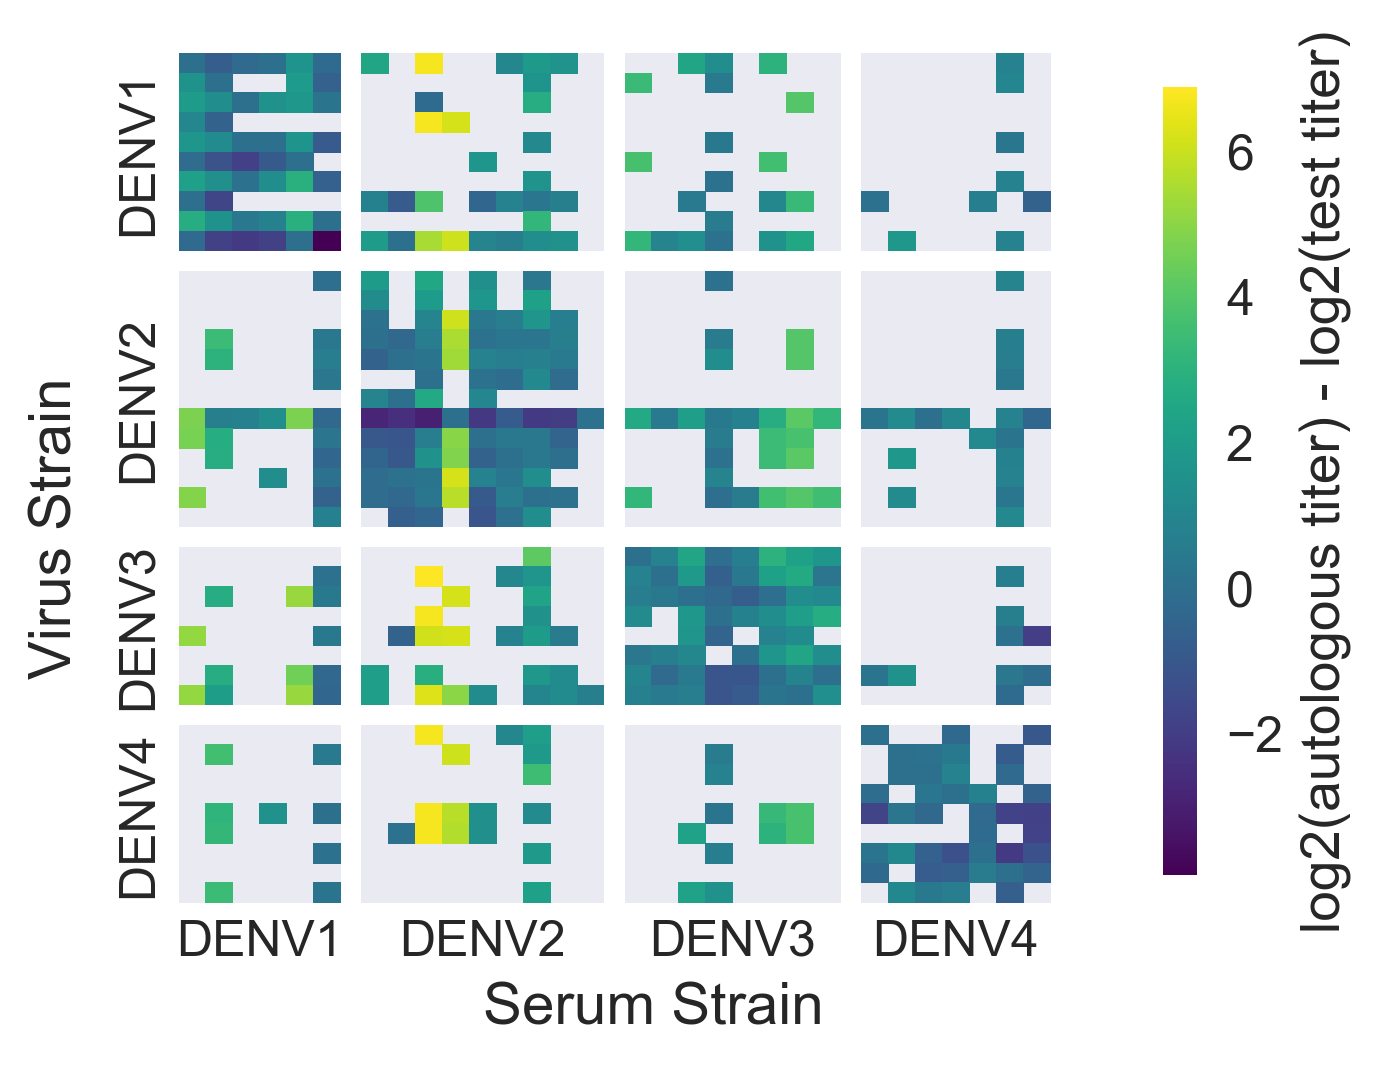
\includegraphics[width=0.7\textwidth]{../figures/png/titer_heatmap.png}
    \caption{\textbf{Normalized antigenic distance between pairs of dengue virus strains and sera.} Neutralization titers from Katzelnick et al. were normalized such that the distance between autologous virus:serum pairs is 0, and each titer unit corresponds to one 2-fold change in PRNT50 value. Light gray areas represent missing data. Higher values correspond to greater antigenic distance.}
     \label{titer_heatmap}
\end{centering}
\end{figure}

The full dataset of normalized titer values is shown in Figure ~\ref{titer_heatmap}.
Here, we see that homotypic virus-serum pairs are more closely related antigenically than heterotypic pairs.
However, we also observe large variance around this trend, both within and between serotypes.
This suggests that treating each serotype as antigenically uniform overlooks potentially important antigenic heterogeneity across strains within each serotype.

\subsection{Dengue antigenic evolution corresponds to phylogenetic divergence}

\begin{figure}[h]
  \begin{centering}
  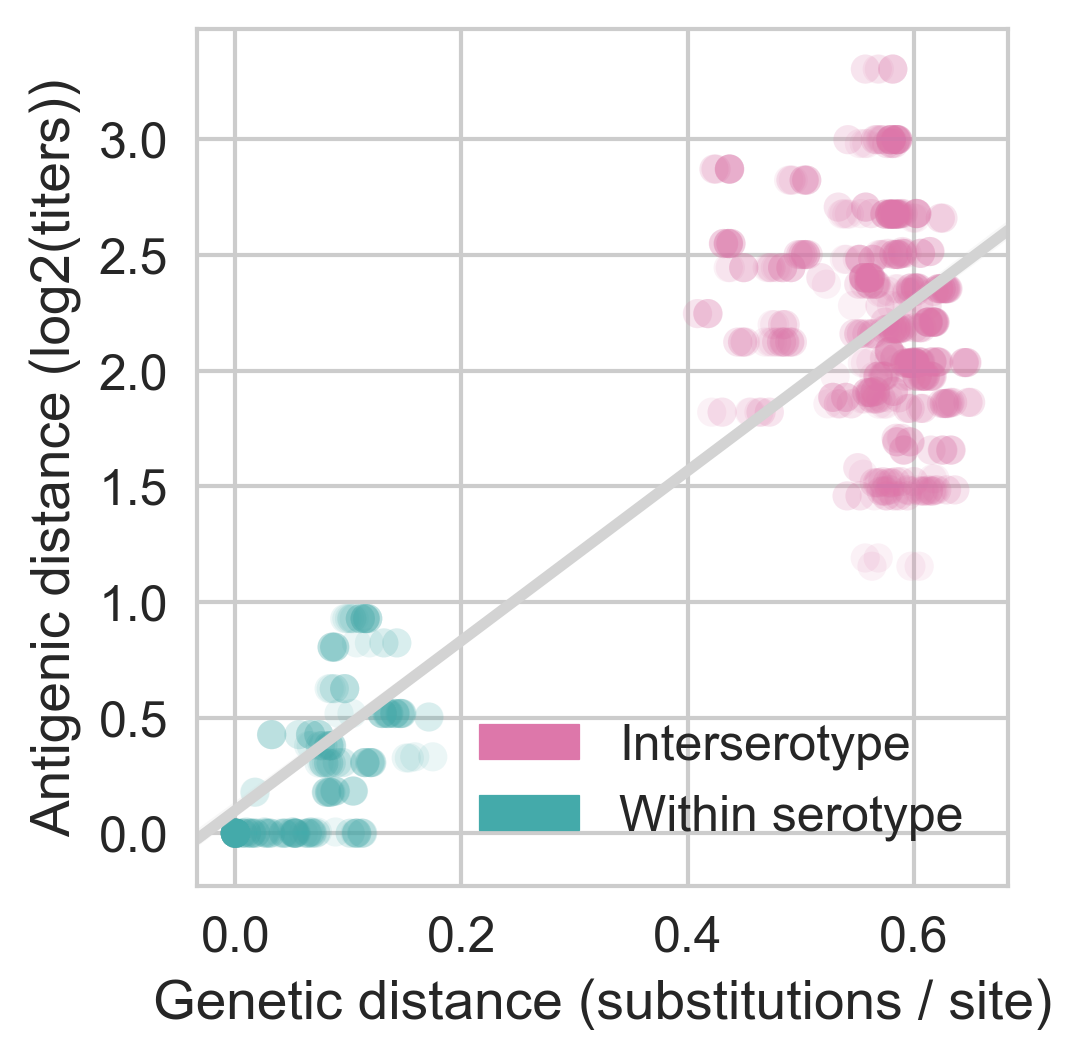
\includegraphics[width=0.6\textwidth]{../figures/png/genetic_antigenic_distance.png}
  	\caption{\textbf{Normalized antigenic distance vs. genetic distance between pairs of dengue strains.}  Normalized antigenic distance between virus strains from Figure 1 as a function of the patristic distance between them on a maximum likelihood phylogeny of viral genomes.}
  	\label{genetic_antigenic_distance}
  \end{centering}
\end{figure}

Titer measurements are prone to noise, and there is a limited amount of available data.
If the antigenic heterogeneity observed in the raw data is truly the result of an underlying evolutionary process, we expect changes in antigenic phenotype to be driven by underlying changes in viral genotype.
Figure ~\ref{genetic_antigenic_distance} shows the relationship between genetic and antigenic distance between each pair of viruses in our dataset.
There are two groups of comparisons --- between serotype and within serotype --- however, even within serotypes there is significant genetic diversity and a correlation between increased genetic distance and increased antigenic distance.
The relationship between genetic distance and antigenic distance is consistent within and between serotypes, where the same trend line can be fit to both within and between comparisons.
Notably, increasing genetic divergence generally corresponds to increased antigenic distance, both within and between serotypes.

\subsection{Within-serotype antigenic evolution better explains observed antigenic relationships}

% SB: This is a weird place for this figure to go, but I can't quite decide where to put it. Thoughts?
\begin{figure}[h]
  \begin{centering}
    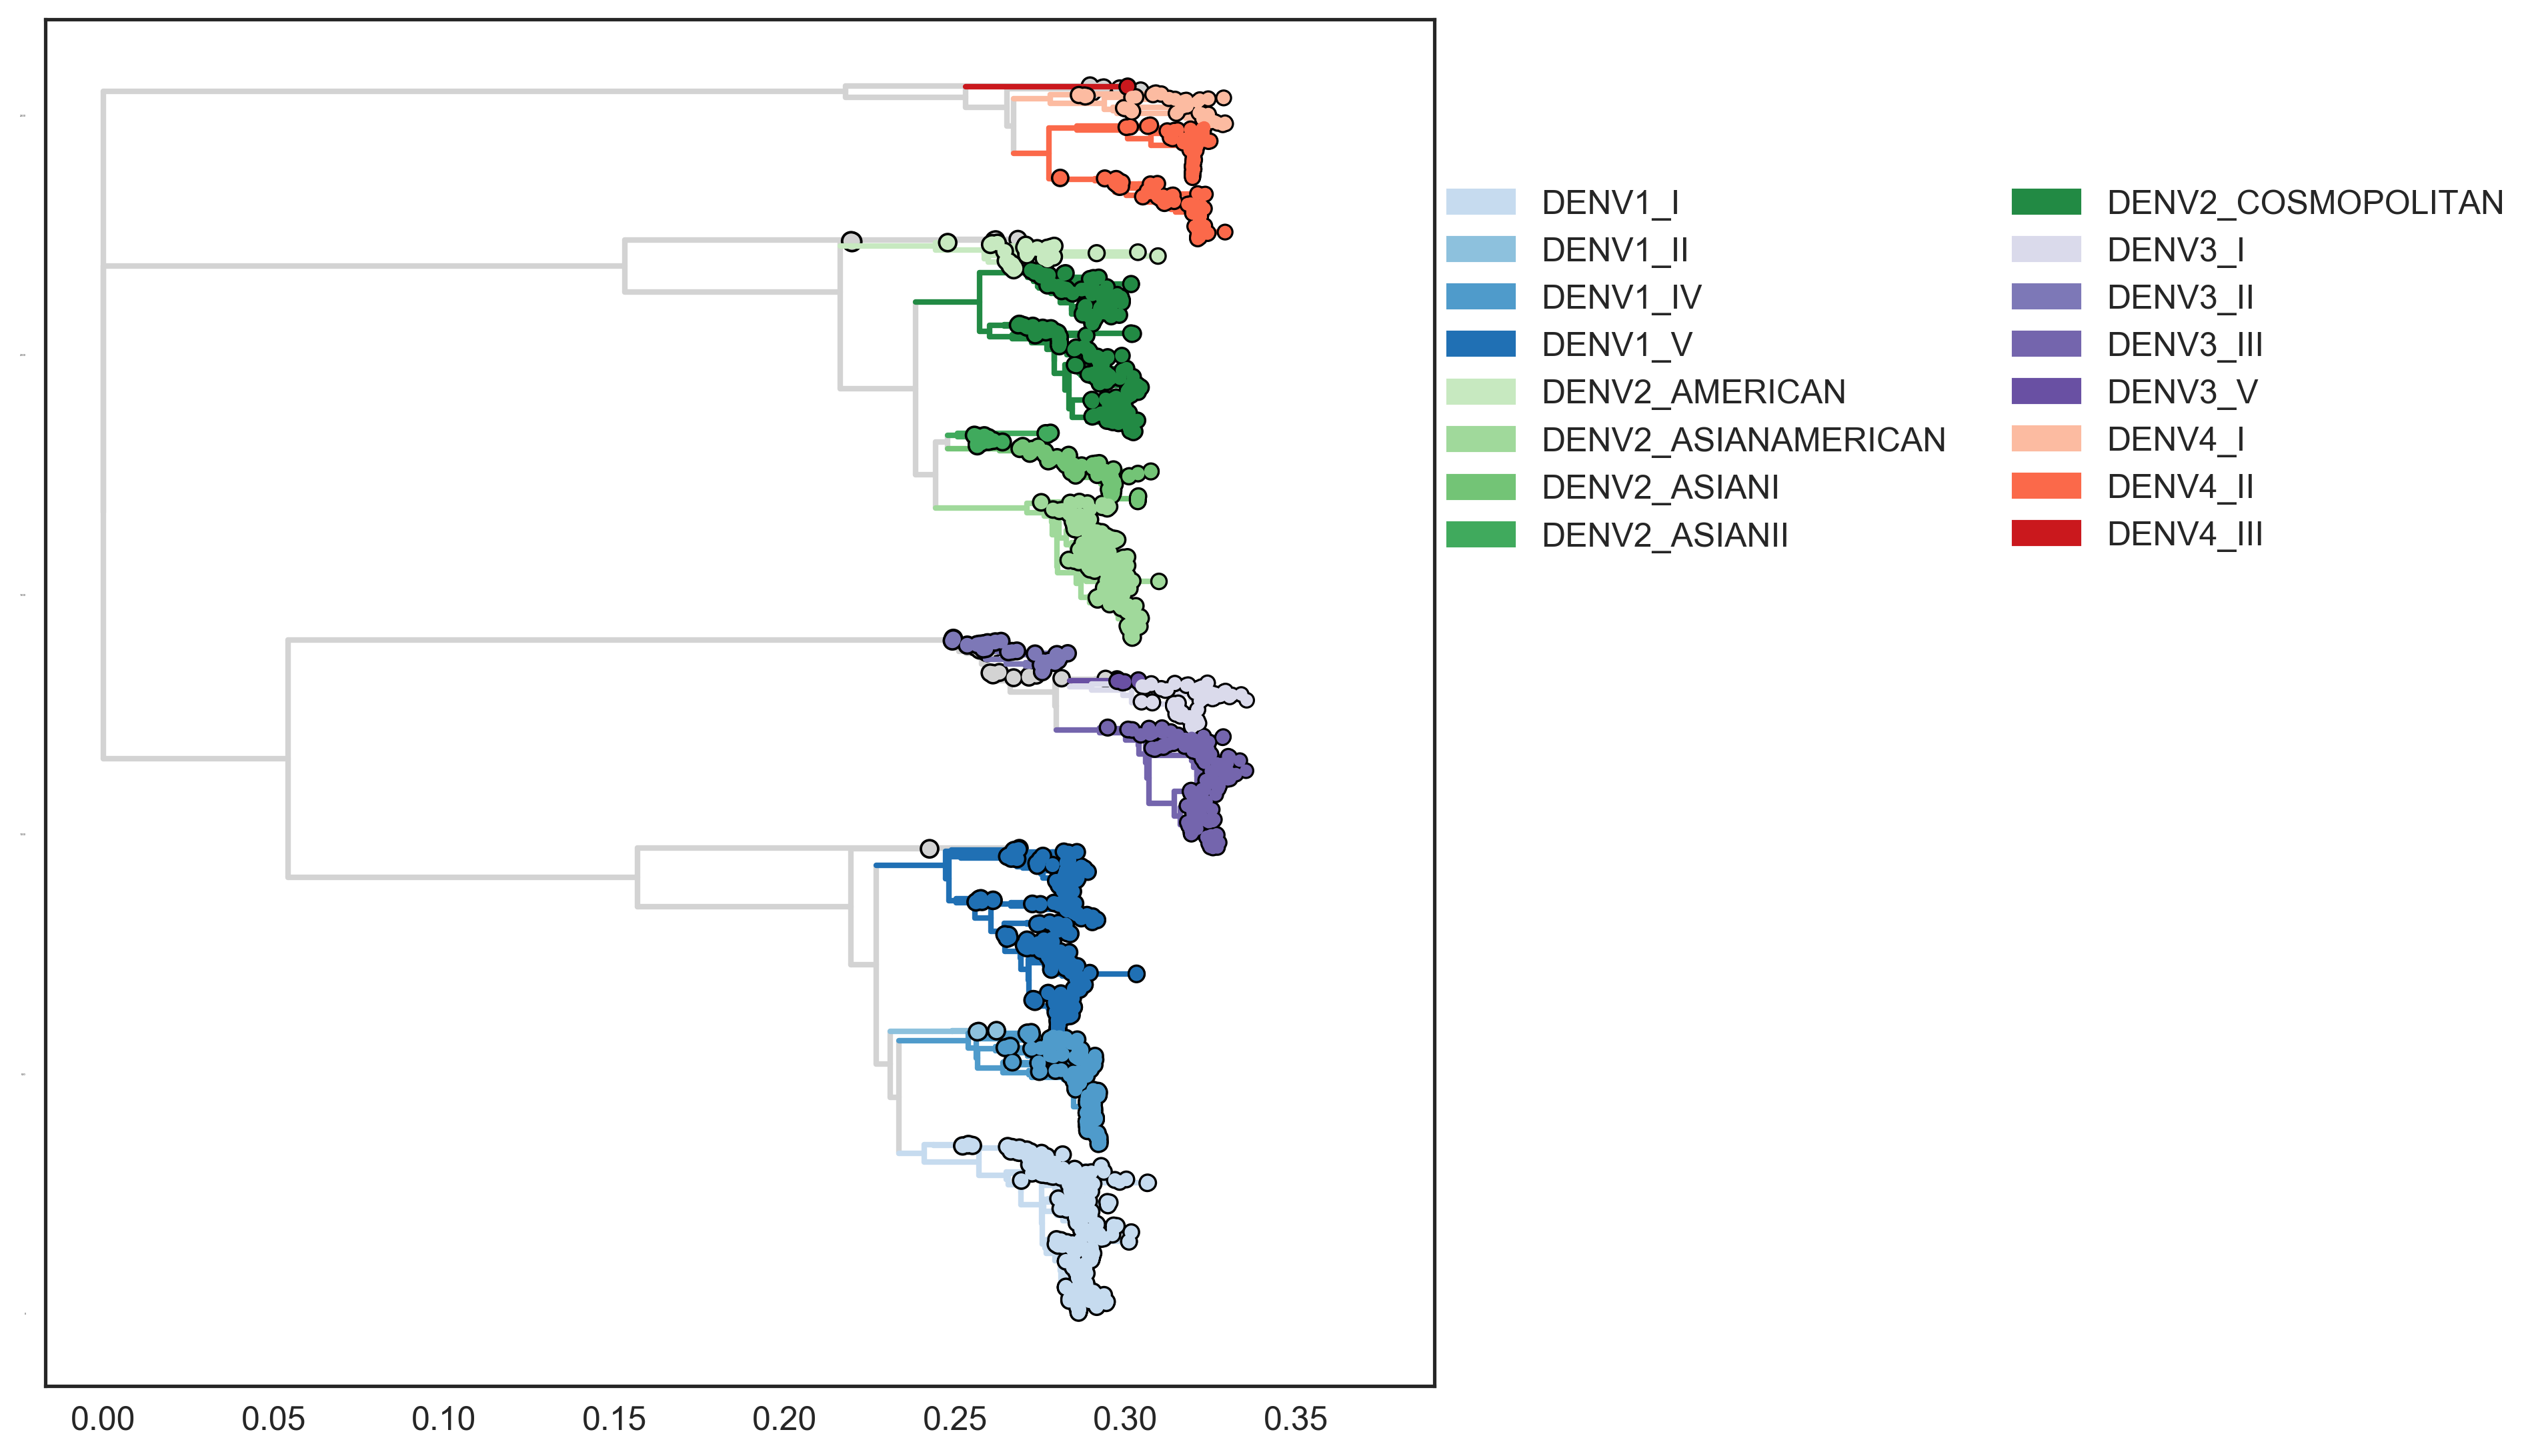
\includegraphics[width=\linewidth]{../figures/png/genotype_tree.png}
  	\caption{\textbf{Phylogeny of dengue viral sequences.}  Maximum likelihood phylogeny of dengue virus genomes, colored by canonical genotype assignment.}
  	\label{genotype_tree}
  \end{centering}
\end{figure}

We then sought to fully map the relationship between DENV genetic and antigenic evolution.
To do so, we adapted a phylogenetics-based model originally developed for influenza.
Conceptually, this model predicts titer values through three steps (see Methods for detailed formulas).
First, we build a phylogeny of dengue virus sequences to establish the genetic relationships between viruses (Figures ~\ref{genotype_tree}, ~\ref{sequence_distribution}).
Next, we infer how much antigenic change has occurred along each branch of the phylogeny.
This assigns each branch $b$ an antigenic distance $d_b$.
With this in hand, we estimate the antigenic distance between any pair of viruses by tracing the path between them in the phylogeny, summing branch-specific distances $d_b$ as we go.

To learn these values of $d_b$, we first split our dataset into training (random 90\% of measurements) and test data (the remaining 10\% of values).
We take the training data and fit $d_b$ for each branch in the tree, subject to regularization.
Parsimoniously, we expect that antigenic change is more likely to occur through fewer, larger changes than through many small changes; correspondingly, values of $d_b$ are exponentially distributed such that most values of $d_b = 0$.
This is analogous to lasso regression to identify a few parameters with positive weights and set other parameters to 0.
Additionally, some viruses have greater binding avidity, and some sera are more potent than others; these row and column effects, respectively, are normally distributed and are taken into account when estimating titers.
The model uses convex optimization to learn the values of $d_b$ that minimize the sum of squared error (SSE) between observed and predicted titers in the training data.

\begin{figure}[h]
  \begin{centering}
    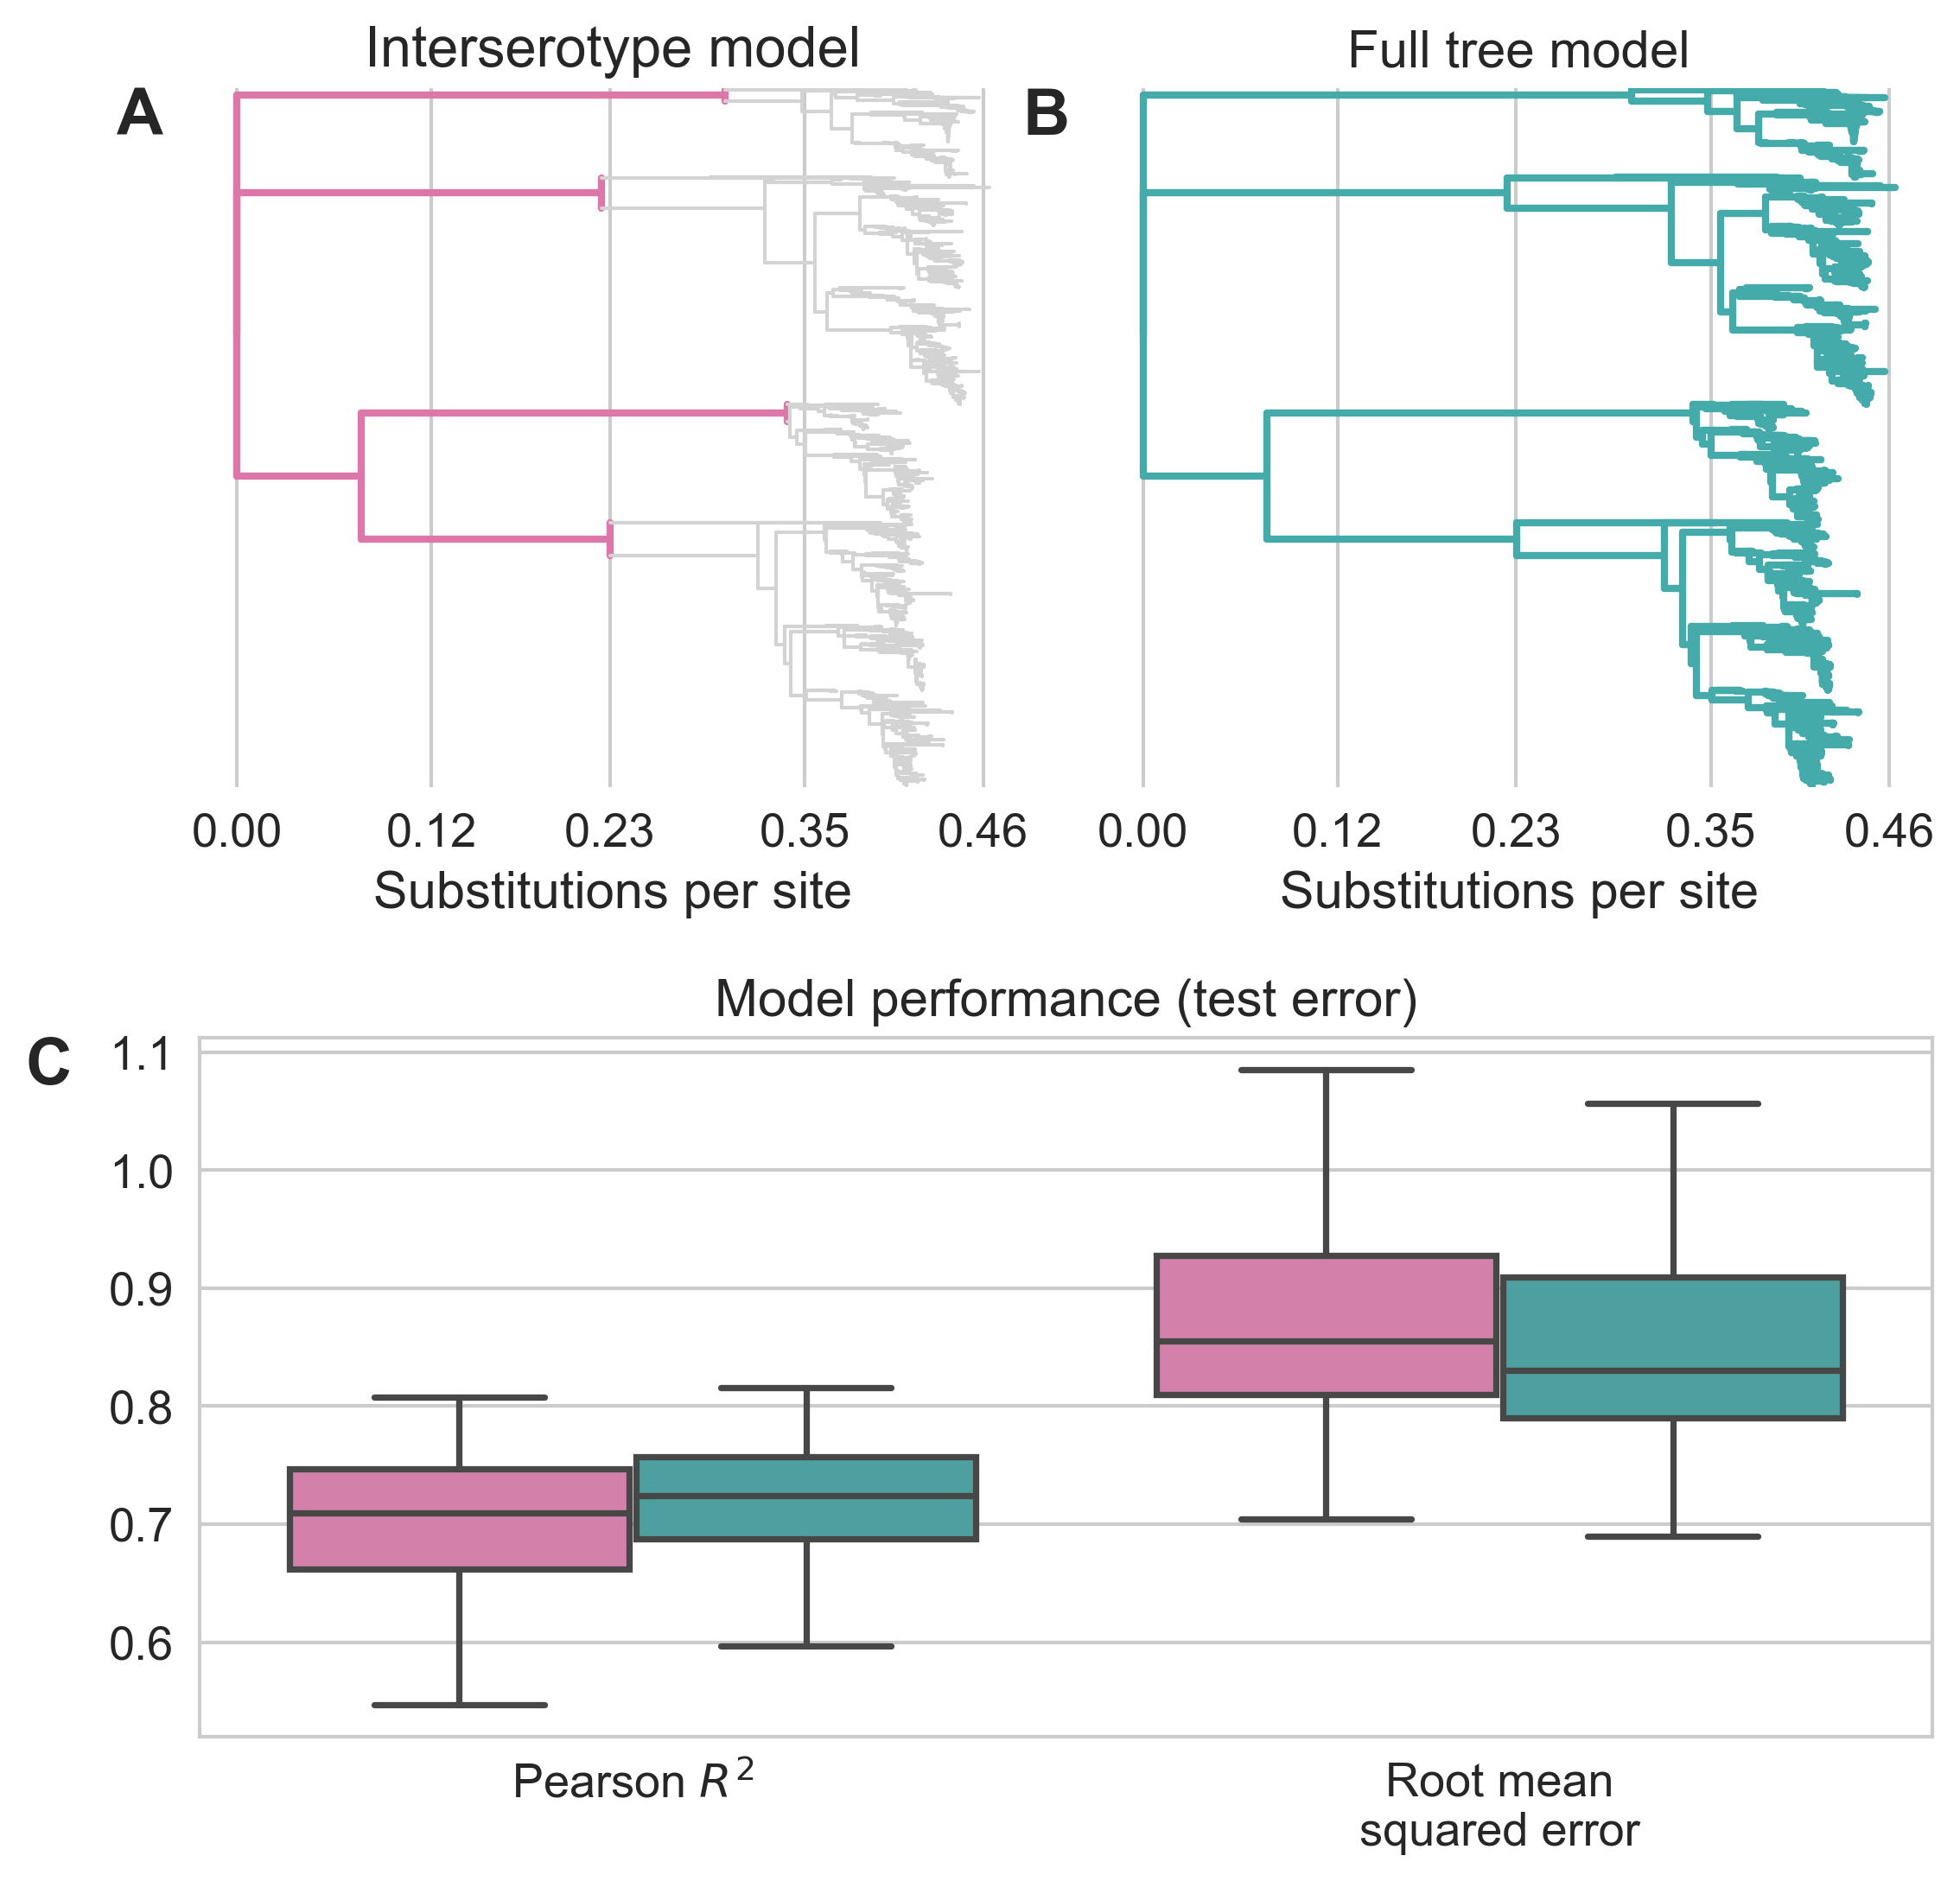
\includegraphics[width=.8\textwidth]{../figures/png/titer_model_performance.png}
        \caption{\textbf{Titer model formulations and performance.}  \textbf{A} The `interserotype model' only allows branches that lie between serotypes to contribute to antigenic evolution. All other branches are assigned $d_b = 0$. \textbf{B} The `full tree model' allows any branch in the phylogeny to contribute to antigenic evolution. \textbf{C,D} Predictive performance of each model on the test dataset (aggregated from 10-fold cross-validation).}
         \label{titer_model_performance}
  \end{centering}
\end{figure}

This model is an effective tool for estimating antigenic relationships between viruses based on their relative positions in the phylogeny.
We can also use variations of this model to explicitly test whether the observed antigenic phenotypes are better explained by the hypothesis that dengue serotypes are antigenically uniform ('interserotype model'), or by the hypothesis that serotypes are antigenically diverse ('full tree model').
In the interserotype model, we set $d_b = 0$ for all branches in the tree that do not lie between serotypes (Figure ~\ref{titer_model_performance}A).
The `full tree model' allows any branch in the phylogeny to contribte to antigenic evolution (Figure ~\ref{titer_model_performance}B).
For each model, we learn model parameters from the training data, and then use those parameters to predict test data values.
We assess model performance by comparing the predicted test titer values to the actual values.
Model performance indicates how well the hypothesis embedded in the model explains the observed data.

We find that serotype-level characterization is insufficient to explain observed antigenic phenotypes.
On average, this interserotype model predicts titers within $1.27$ $log_2$ titer units of the true value (root mean squared error, RMSE), and explains $22\%$ of the observed variation in neutralization titers overall (Figure ~\ref{titer_model_performance}).

We find that accounting for within-serotype antigenic evolution substantially improves our ability to explain dengue antigenic phenotypes.
The full tree model is able to predict test titers within $0.89$ $log_2$ titer units of the true value (RMSE approaching the level of error intrinsic to the assay), and explains $66\%$ of the observed variation in neutralization titers overall (Figure ~\ref{titer_model_performance}).
Importantly, all reported error metrics refer to performance on test data, so this difference in model performance is not due to the number of free parameters.
The full tree model performance is comparable to the model error from a cartography-based characterization of the same dataset (RMSE $0.65-0.8$ $log_2$ titer units), and to the error observed when this model was used to characterize an influenza dataset (RMSE of $0.5$ $log_2$ titer units).
From this, we conclude that there is antigenic evolution within each serotype of DENV, and that this is driven by underlying genetic divergence.

\subsection{There are at least 12 distinct antigenic phenotypes of dengue}

% I'm not sure I actually like this figure, but I can't think of a better representation.
\begin{figure}[h]
  \begin{centering}
    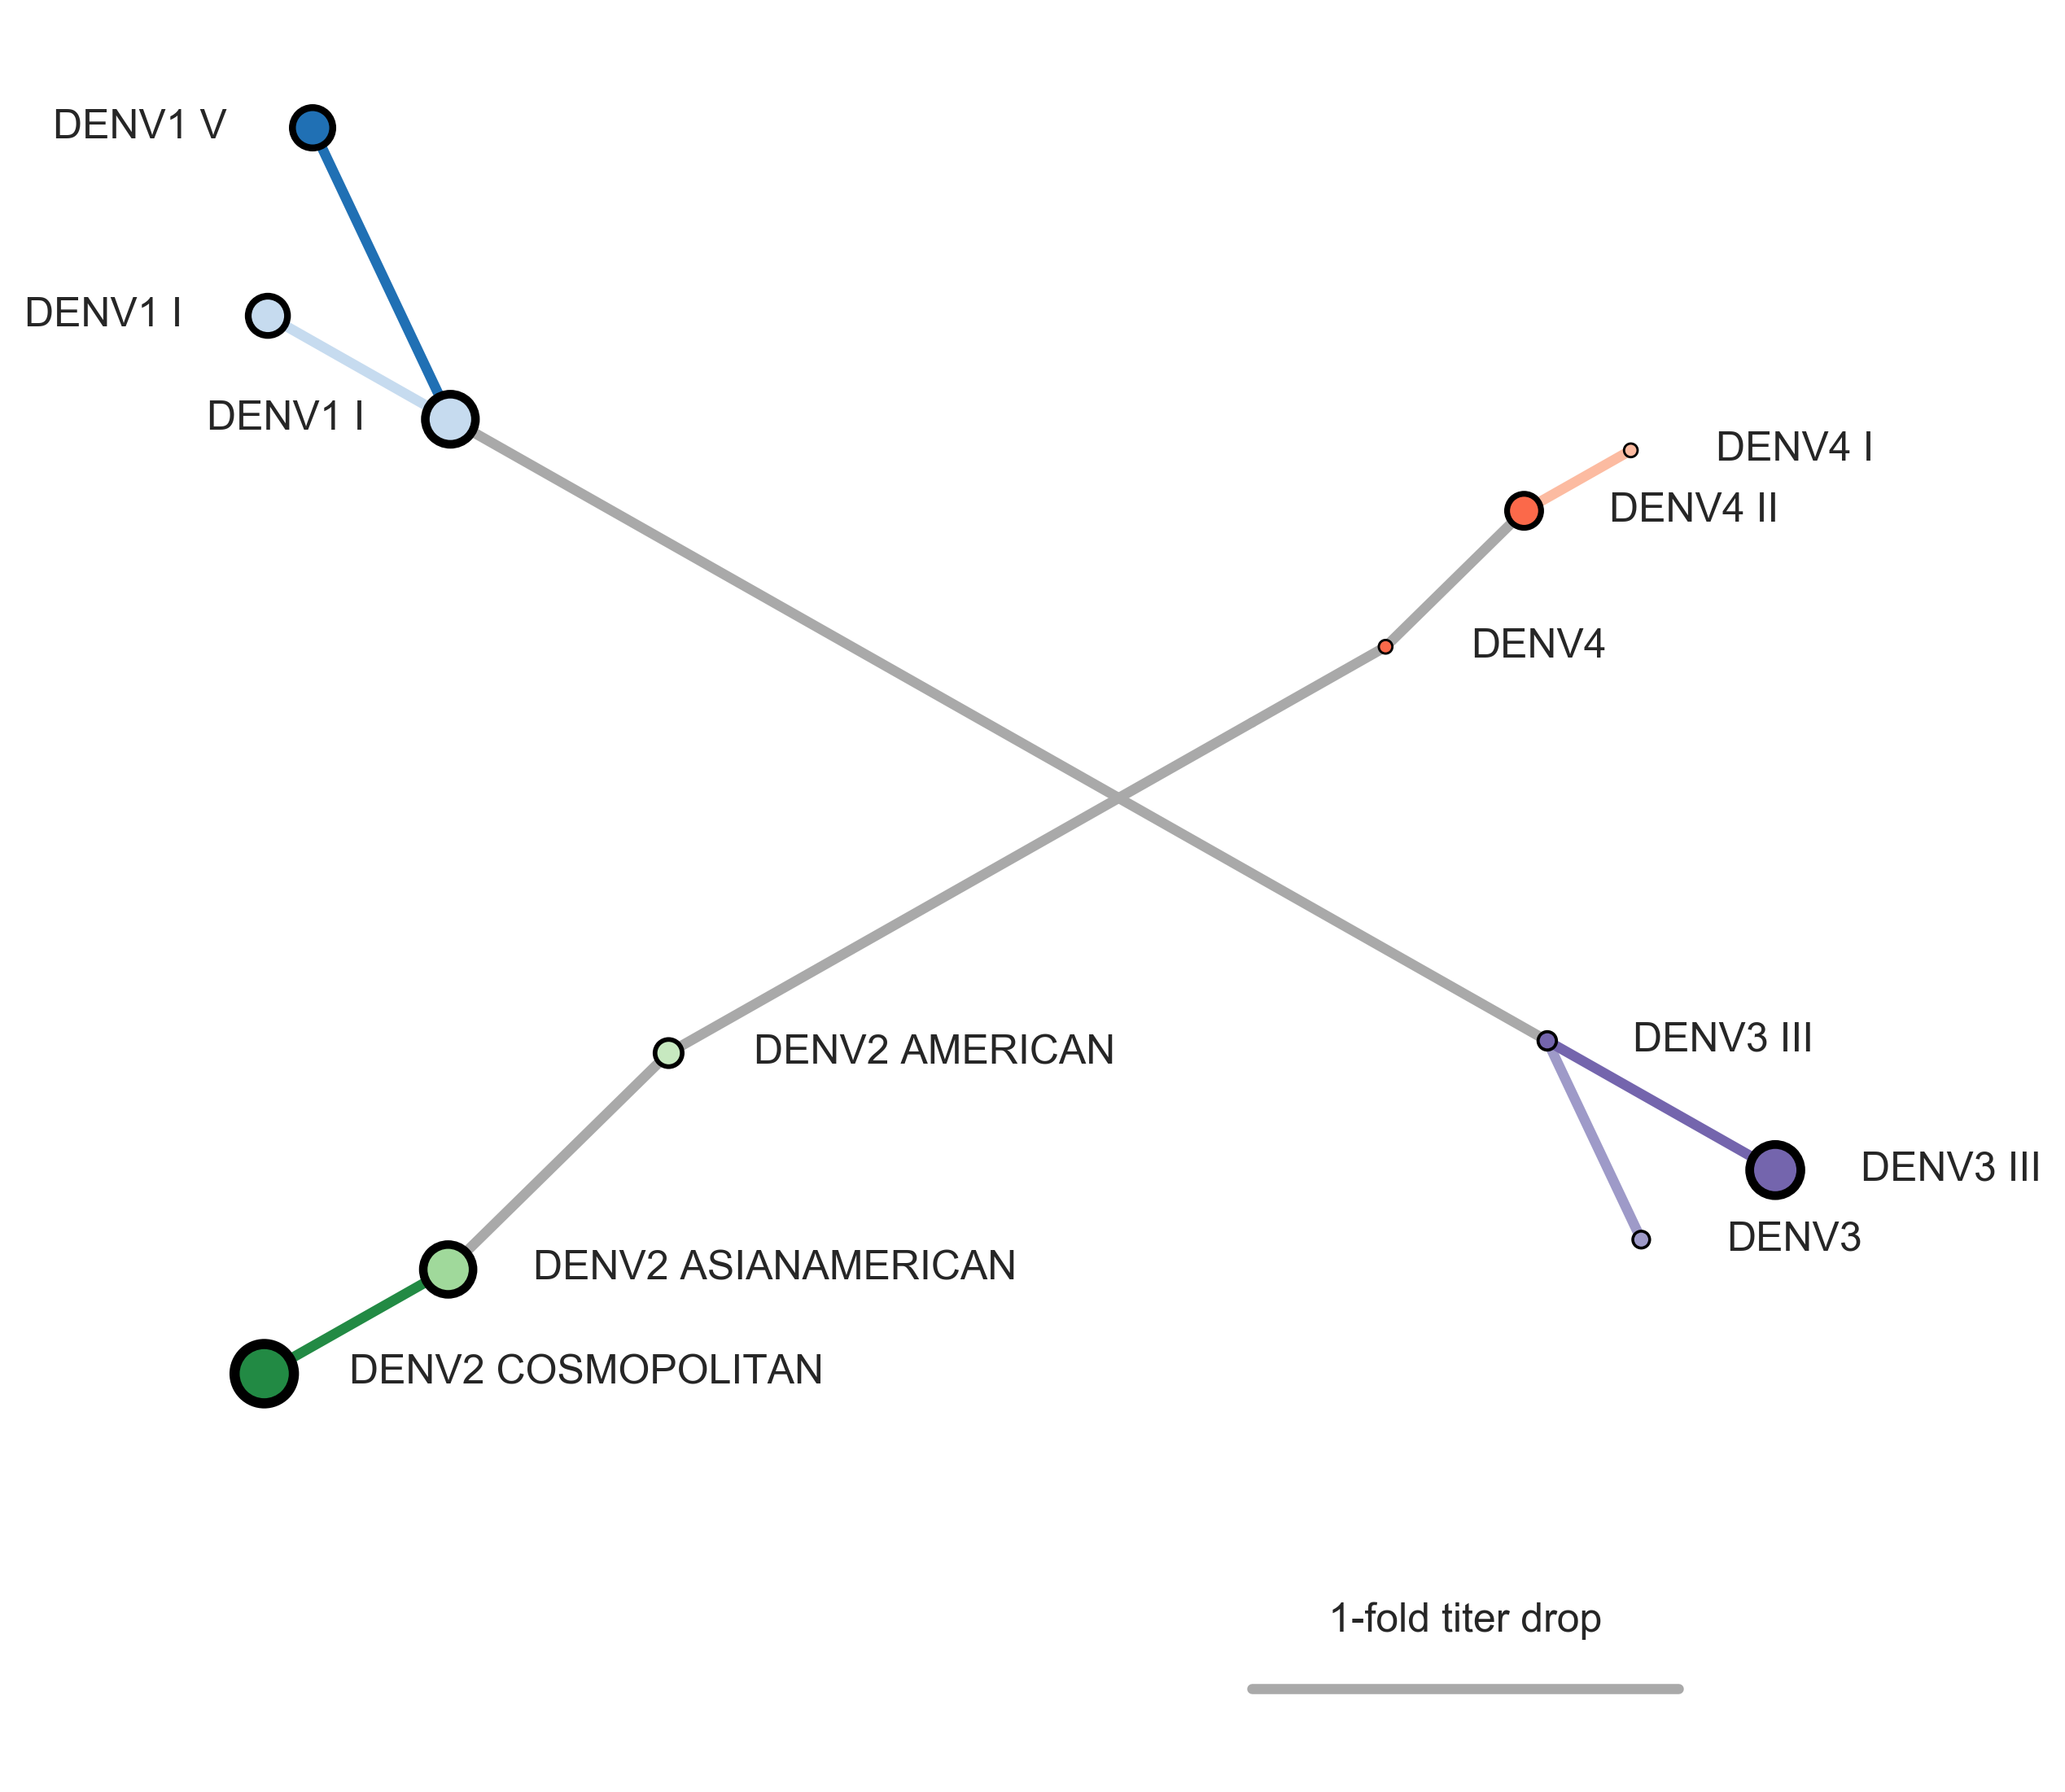
\includegraphics[width=.8\linewidth]{../figures/png/antigenic_tree.png}
    \caption{\textbf{Tree of dengue antigenic phenotypes.}  A maximum likelihood phylogeny of DENV genomes was used to infer the topology, with branch lengths scaled to reflect $d_b$, the relative contributions of each branch to antigenic divergence, as inferred by the `full tree model'. Antigenically uniform clades were collapsed, and node sizes reflect the size of the collapsed clade.}
     \label{antigenic_tree}
  \end{centering}
\end{figure}

Collapsing putatively antigenically uniform clades, we observe at least 12 distinct antigenic phenotypes of dengue (Figure ~\ref{antigenic_tree}).
The titer dataset spans the breadth of canonical DENV genotypes, but in most cases lacks the resolution to detect within-genotype antigenic diversity (Figure ~\ref{genotype_dTiter_heatmap}).
We thus expect that these results represent a lower-bound on the true extent of DENV intraserotype antigenic diversity, but these results clearly reject the null hypothesis that all DENV strains within a serotype are antigenically uniform.

\subsection{Antigenic novelty predicts serotype success}
We observe strong evidence that homotypic genotypes of dengue vary in their ability to escape antibody neutralization.
However, antibody neutralization is only one of many factors that contribute to secondary infection outcomes.
We thus wanted to know whether the observed antigenic diversity influences dengue population dynamics in the real world.
At any given time, many factors contribute to both the total size of the viral population (which corresponds to the incidence in the host population), and the makeup of the viral population (the relative frequency of each viral strain currently circulating).
For example, seasonal fluctuations in mosquito population size and many other environmental factors influence the DENV population size.
The relative makeup of this viral population is strongly driven by viral fitness.
In meaningfully antigenically diverse viral populations, antigenic novelty contributes to viral fitness: as a given virus $i$ circulates in a population, the proportion of the population that is susceptible to infection with $i$--and other strains antigenically similar to $i$--decreases over time as more people acquire immunity.
Antigenically novel viruses that are able to escape this population immunity are better able to infect hosts, making them fitter than the previously circulating strain.
Thus, if antigenic novelty constitutes a fitness advantage for DENV, then we would expect greater antigenic distance from recently circulating strains to correlate with higher growth rates.

\begin{figure}[h]
  \begin{centering}
    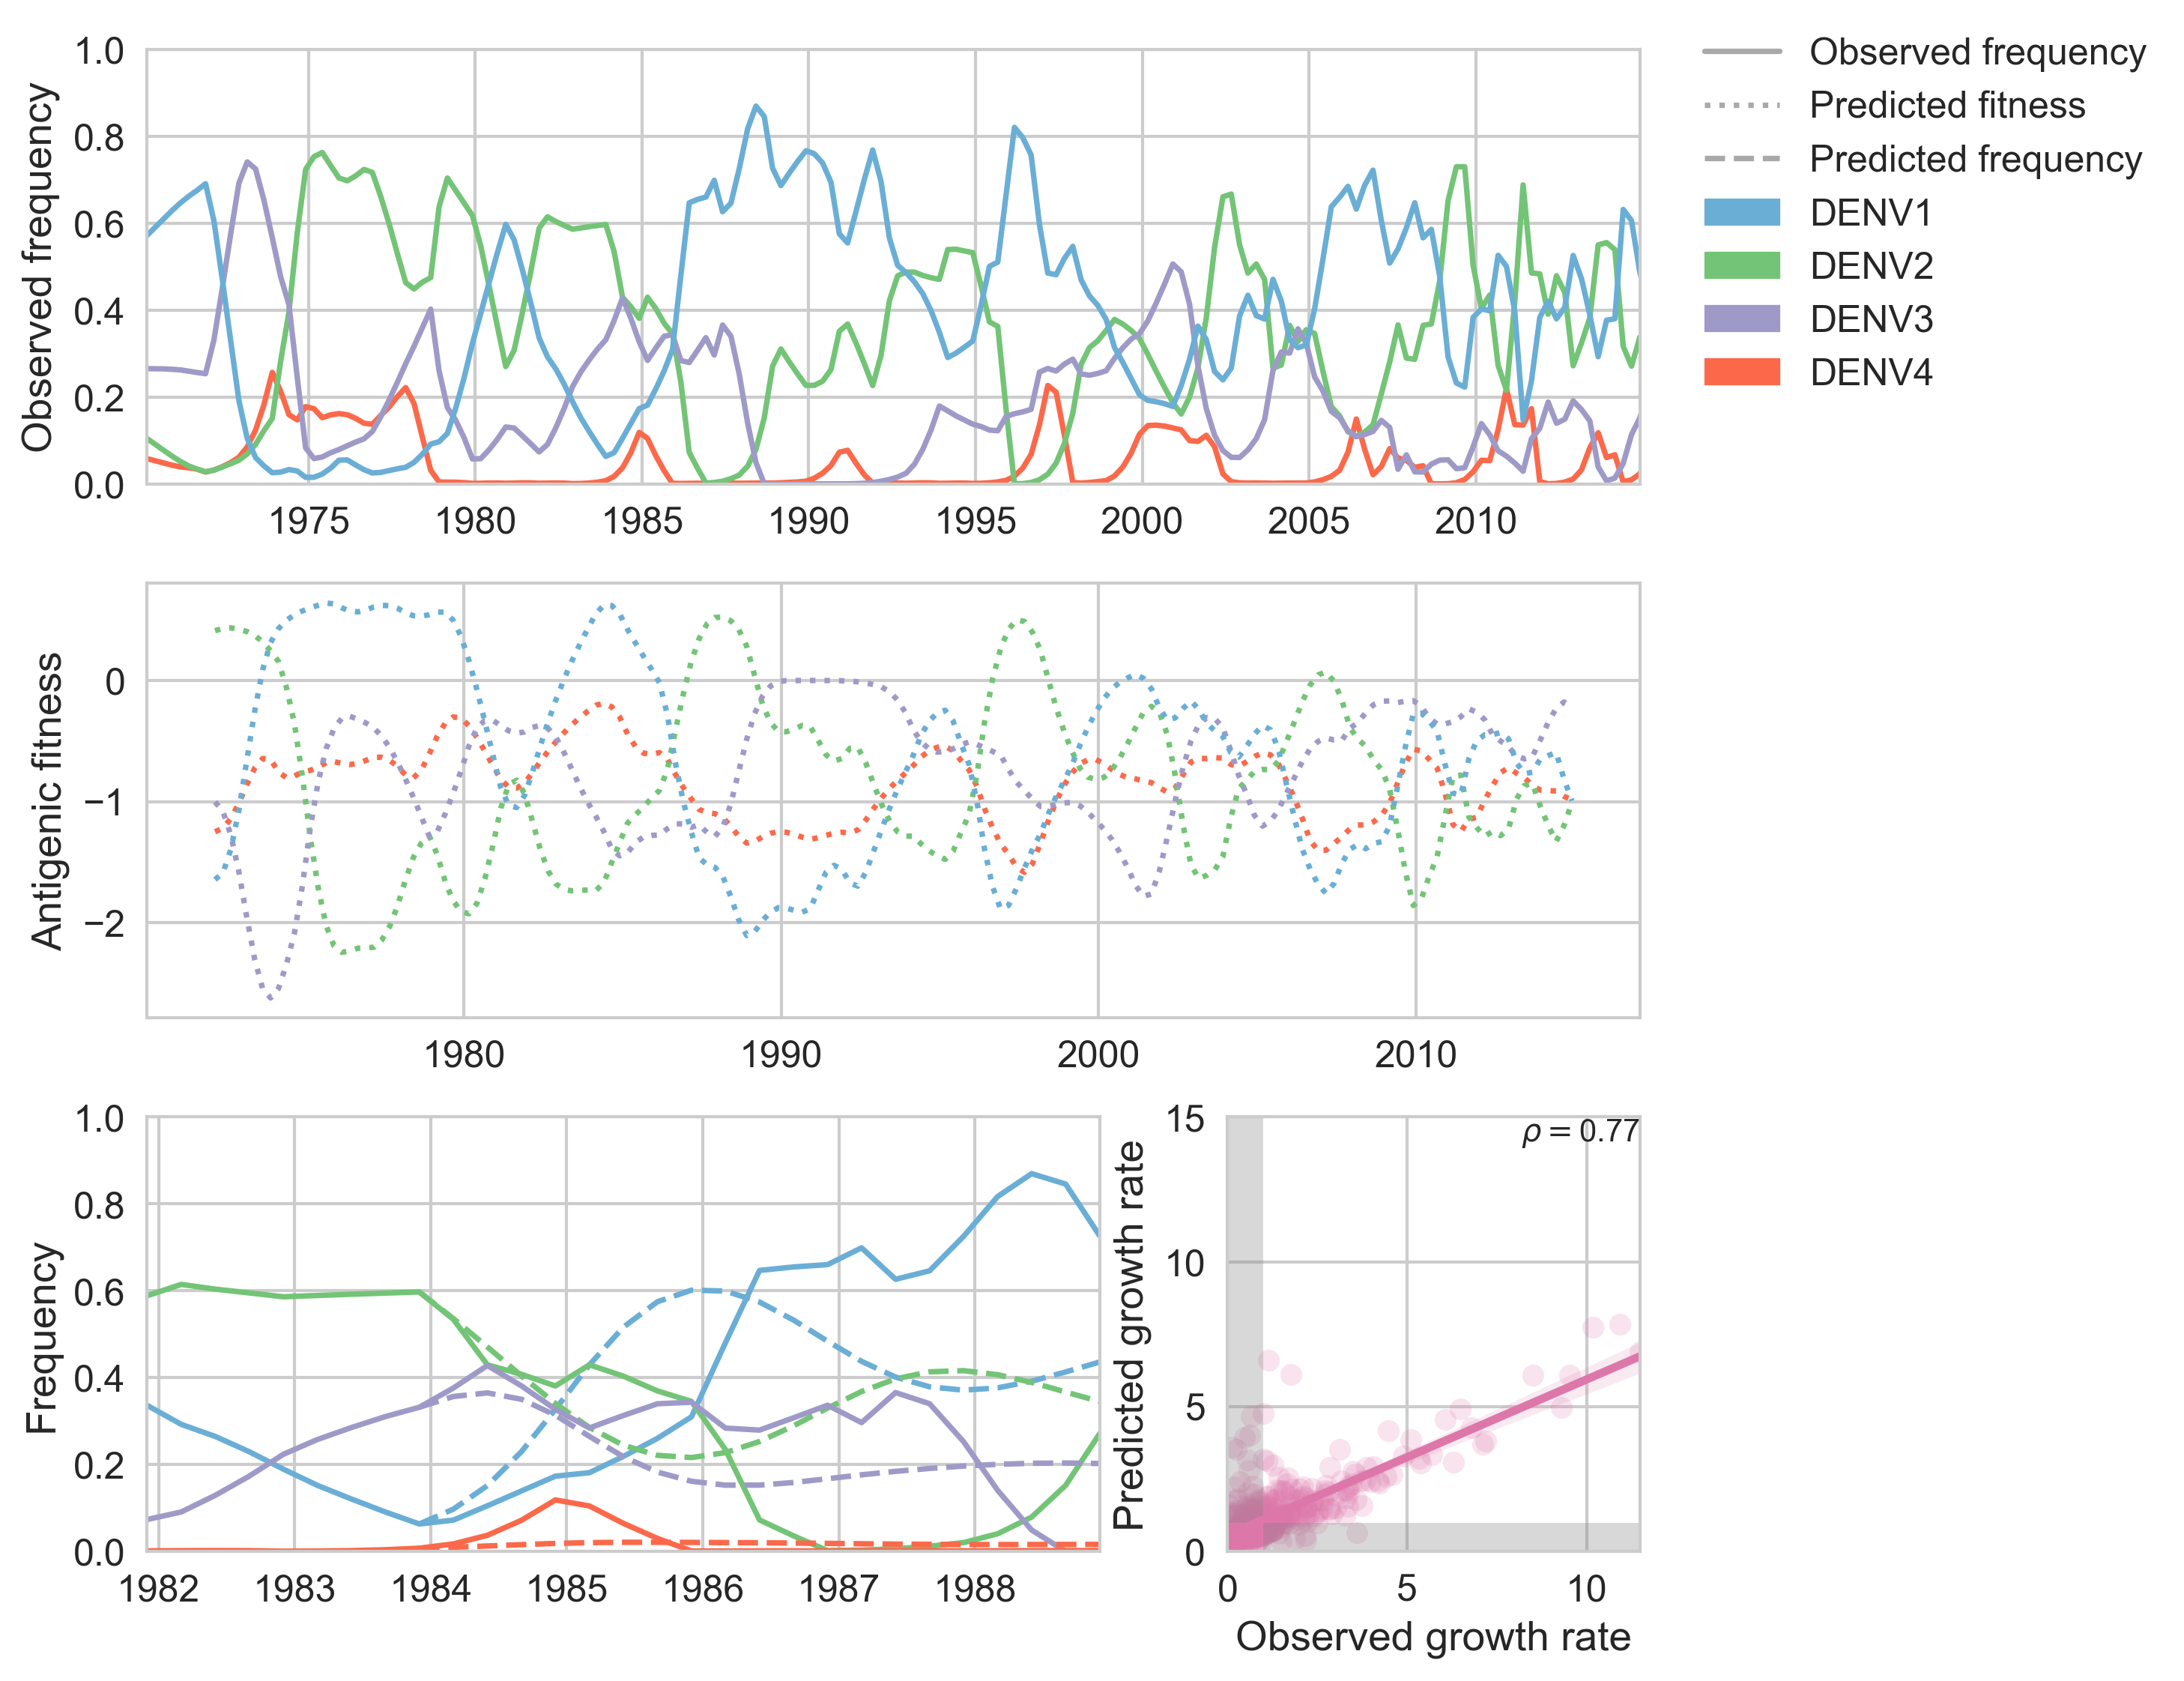
\includegraphics[width=\linewidth]{../figures/png/serotype_fitness_model.png}
  	\caption{\textbf{Antigenic novelty predicts serotype success.}  \textbf{A} The relative frequency of each serotype in Southeast Asia was estimated every 3 months based on available sequence data. \textbf{B} At each timepoint, we calculate the relative fitness of each serotype based on its antigenic novelty (frequency-weighted distance from recently circulating strains) and a scaling factor representing the intrinsic fitness of each serotype. \textbf{C} At each timepoint $t$, we blind the model to all empirical data from timepoints later than $t$ and predict each clade's future trajectory based on its initial frequency and antigenic fitness at time $t$; we predict forward in 3-month increments, compounding population immunitiy and adjusting antigenic fitness based on predicted frequency changes, for a total prediction period of $dt = 5 years$. \textbf{D} Predicted growth rates are calculated as $\frac{\hat{x_i}(t+dt)}{x_i}(t)$ and compared to empirically observed growth rates. Clade growth versus decline is accurate for 80\% of predictions (points outside the shaded gray area).}
  	\label{serotype_fitness_model}
  \end{centering}
\end{figure}

To test this hypothesis, we examined the makeup of the dengue virus population in Southeast Asia from 1970 to 2015.
We estimated the relative population frequency of each DENV serotype at 3-month intervals, $x_i(t)$ (Figure ~\ref{serotype_fitness_model}A), based on available sequence data (see Methods).

Fitter viruses increase in population frequency over time, such that $x_i(t+dt) > x_i(t)$.
It follows that these viruses have a growth rate--defined as the fold-change in frequency over time--greater than 1: $\frac{x_i(t+dt)}{x_i(t)} > 1$.
To isolate the extent to which antigenic novelty contributes to clade success and decline, we built a simple model that attempts to predict clade growth rates based on two variables: the antigenic fitness of the clade at time $t$, and a time-invariant fit parameter representing the intrinsic fitness of the serotype the clade belongs to.
Growth rates are estimated based on a 5-year sliding window (Figure ~\ref{serotype_fitness_model}C).
We estimate the antigenic fitness of virus $i$ at time $t$ as a function of its antigenic distance from each strain $j$ that has circulated in the same population over the previous two years, weighted by the relative frequency of $j$ and adjusted for waning immunity (Figure ~\ref{serotype_fitness_model}B; see Methods).
Serotype intrinsic fitness is a free parameter and is constant over time.

This simple model explains 62\% of the observed variation in serotype growth rates, and predicts serotype growth vs decline correctly for 80\% of predictions (Figure ~\ref{serotype_fitness_model}D).
This strongly suggests that antigenic novelty is a major driver of serotype population dynamics. % add an estimate here of the relative contribution of antigenic vs. intrinsic fitness
This also demonstrates that this model captures key components of dengue population dynamics, performing significantly better than the null model under which all clades have equal antigenic fitness (see Methods).
Interestingly, the model performs best when we model immunity as waning linearly over time, with the probability of protection dropping by about 48\% per year for the first two years after primary infection.
% add a sentence here about the relative intrinsic fitness values; compare to experimental estimates of replicative fitness

\subsection{Antigenic novelty also partially predicts genotype success}
To directly examine the impact of antigenic fitness on these finer resolution population dynamics, we estimated the relative frequency of each genotype over the same time period.

% fix the x axis here so the subplots line up
\begin{figure}[h]
  \begin{centering}
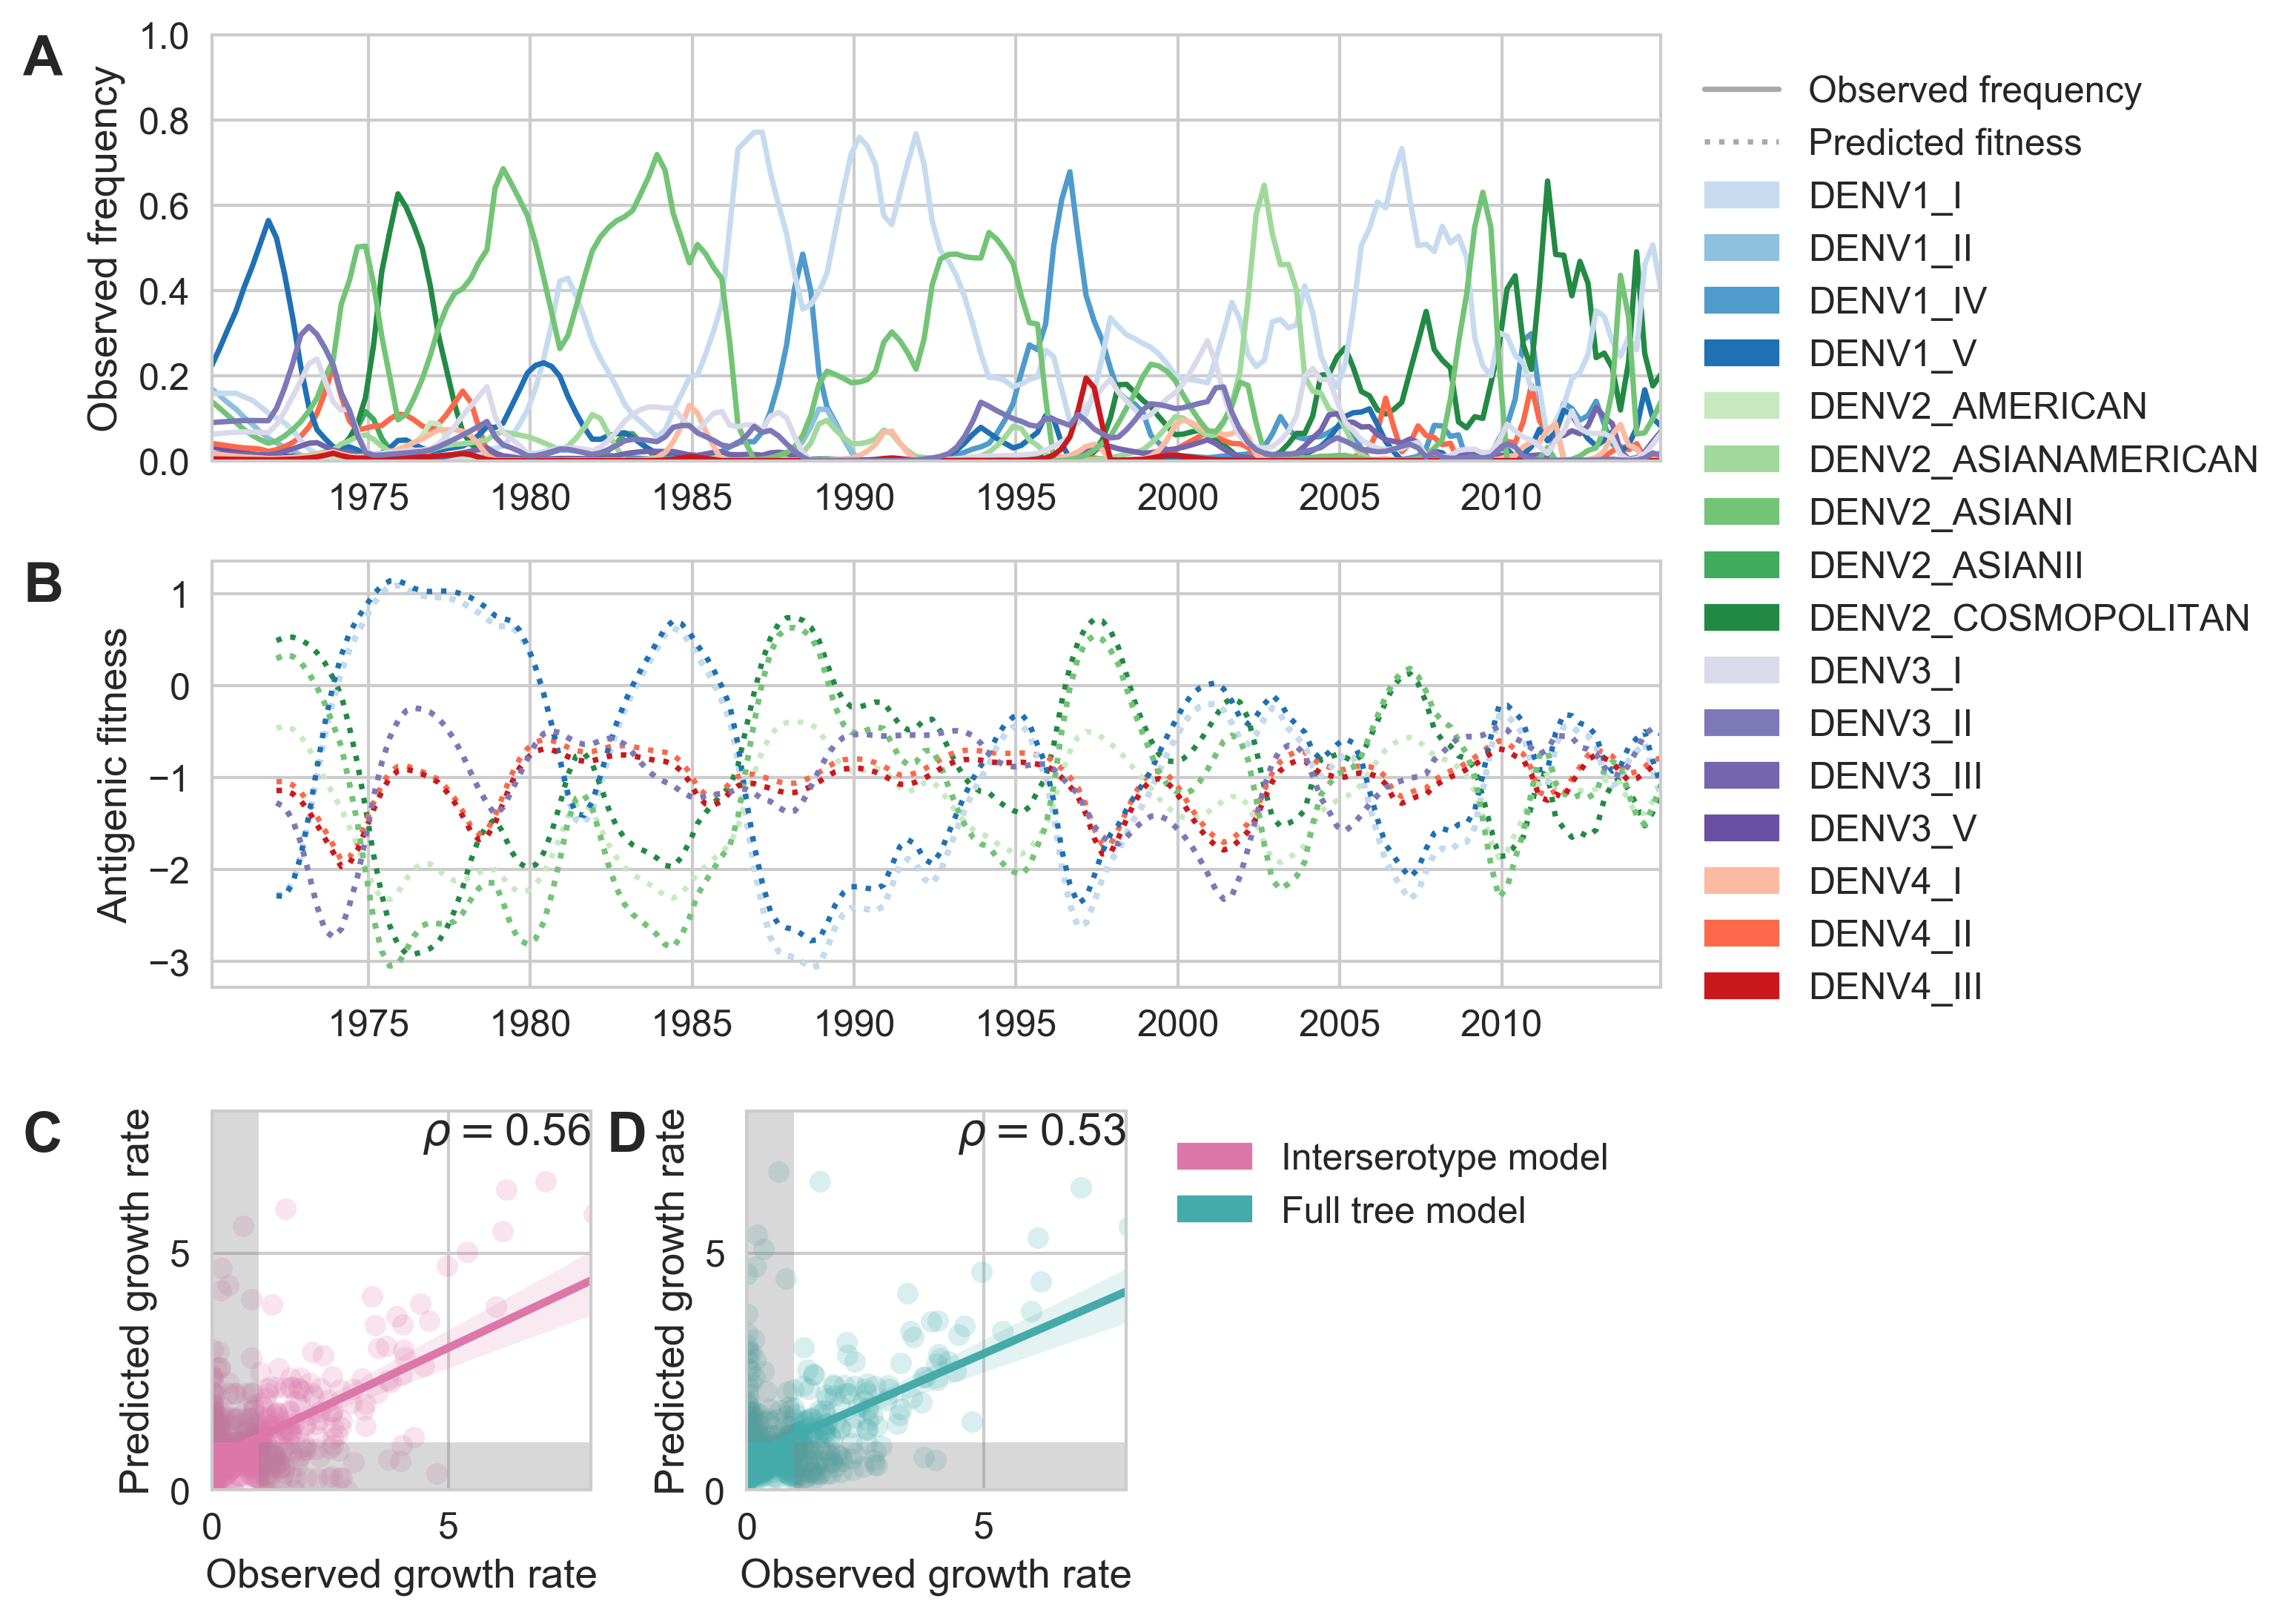
\includegraphics[width=\linewidth]{../figures/png/genotype-fitness.png}
    \caption{\textbf{Relative frequencies and fitness of dengue genotypes, 1970-2015.}  \textbf{A} Relative frequencies of each canonical dengue genotype across Southeast Asia, estimated from available sequence data. \textbf{B} Antigenic fitness was calculated for each canonical dengue genotype as its frequency-weighted antigenic distance from recently circulating strains (here, using antigenic distances estimated from the `full tree model' of antigenic relationships)}
     \label{genotype_fitness}
   \end{centering}
\end{figure}

To estimate how well antigenic novelty predicts genotype success, we used the same model to predict genotype success and decline.
As before, fitness of genotype $i$ is based on the intrinsic fitness of the serotype $i$ belongs to, and the antigenic distance between $i$ and each other genotype, $j$, that has recently circulated (Figure ~\ref{genotype_fitness}).
Importantly, we can calculate antigenic distance between $i$ and $j$ at the serotype level (i.e., the antigenic distances computed from the `interserotype model' above) or at the genotype level (i.e., the antigenic distances computed by the `full tree model', which incoporates the observed within-serotype heterogeneity).
If within-serotype antigenic heterogeneity contributes to genotype fitness, then we would expect the `full tree model' to predict genotype growth rates better than the `interserotype model'.

\begin{figure}[h]
\centering
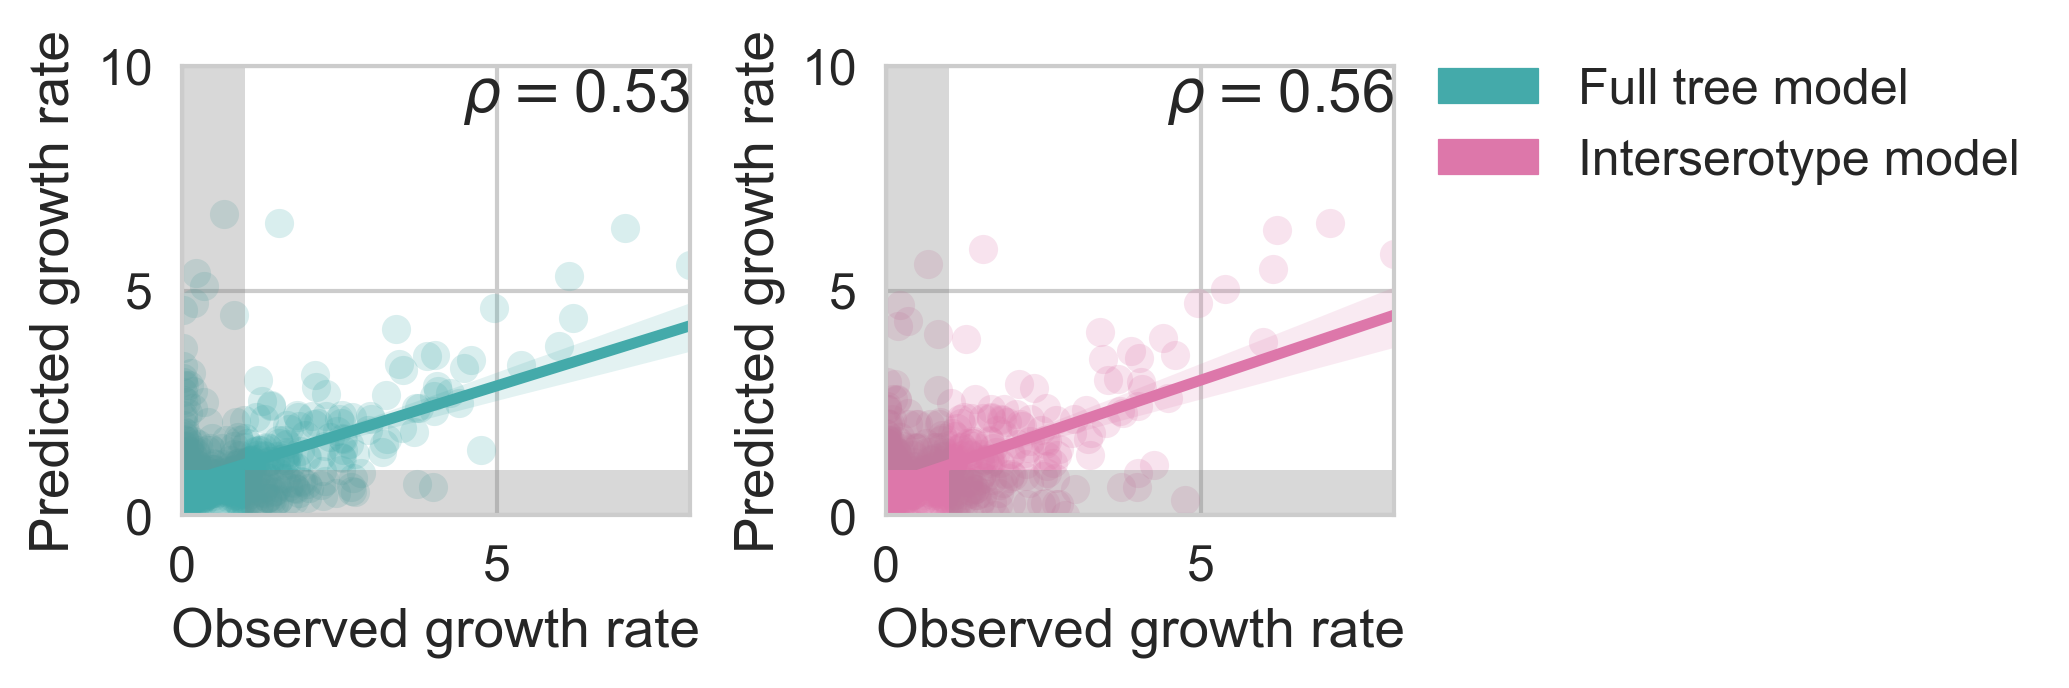
\includegraphics[width=0.7\linewidth]{../figures/png/genotype_growth_rates.png}
\begin{centering}
    \caption{\textbf{Predicted vs. actual genotype growth rates under full-tree or interserotype models of antigenic phenotype.}  Antigenic distance between each pair of canonical genotypes was estimated from either the `full tree model' or the `interserotype model' of antigenic divergence. For each model, antigenic fitness was estimated at each timepoint based on frequency-weighted antigenic distance from recently circulating strains and used to predict genotype growth or decline over a 5-year period.}
     \label{genotype_growth_rates}
\end{centering}
\end{figure}

Overall, we find that antigenic novelty contributes to genotype turnover, although it explains less of the observed variation (Figure ~\ref{genotype_growth_rates}A).
When antigenic distance is estimated from the `interserotype model', we find that antigenic fitness explains approximately 31\% of the observed variation in genotype growth rates, and correctly predicts genotype growth vs. decline 68\% of the time.
% For genotypes, we find that antigenic fitness determines approximately X\% of total fitness.
Surprisingly, more precise estimates of antigenic distance between genotypes from the `full tree model' does not improve our predictions of genotype success ($R^2 = 0.28$, 70\% accuracy; Figure ~\ref{genotype_growth_rates}B).

\section*{Discussion}

\subsection*{Within-serotype antigenic heterogeneity}
We show that mapping antigenic change to individual branches and interpolating across the DENV phylogeny is able to explain a large majority of the observed variation in antigenic phenotypes as measured by neutralization titers.
This suggests that DENV antigenic evolution is closely coupled to genetic divergence.
% This might be a natural spot to discuss why we don't have the statistical power to identify associations between specific mutations and antigenic change.
We also find that accounting for within-serotype antigenic evolution is necessary to explain the observed variation in antigenic phenotypes.
This supports and expands upon previous reports that the null hypothesis of antigenically uniform serotypes is inconsistent with available data.
We observe at least 12 distinct antigenic phenotypes that are both genetically and antigenically distinct.
On average, intraserotype antigenic phenotypes are 0.42 titer units apart and interserotype antigenic phenotypes are 1.78 titer units apart.
For context, analysis of the recent CYD-TDV vaccine trial shows different vaccine efficacy against genotypes I and II of DENV4, which are 0.4 log2 titer units apart in our dataset.
This suggests that the 12 phenotypes we report may be sufficiently distinct to have important impacts on secondary case outcomes and vaccine efficacy.

Overall, we expect that these antigenic phenotypes represent a lower-bound on the extent, magnitude, and nature of antigenic heterogeneity with DENV.
Our current titer dataset spans the breadth of DENV diversity, but in most cases lacks the resolution to detect sub-genotype antigenic variation or to identify which specific mutations correspond to changes in antigenic phenotype.
The appearance of the deep antigenic divergence of the four serotypes, and the more recent antigenic divergences within each serotype, suggest that DENV antigenic evolution is likely an ongoing, though gradual, process.
We therefore expect that future studies with richer datasets will find additional antigenic variation within each genotype.
This dataset also contains many left-censored titer values, where we know two strains are at least N titer units apart, but do not know exactly how far apart.
If we knew the true value of these censored titers, many of them would indicate larger antigenic distances than the reported values used to train the model.
Thus, it is likely that our model systematically underestimates the magnitude of titer distances.
Finally, antibody neutralization and escape (as measured by PRNT titers) is only one component of the immune response to DENV.
Analysis of a longitudinal cohort study shows that these neutralization titers correlate with protection from severe secondary infection, it is important to note that
DENV case outcomes are also mediated by interactions with innate and T-cell immunity, the effects of which are not captured in neutralization titers. % the fact that titer-based estimation of antigenic fitness is predictive of clade dynamics provides additional validation of neuts as a measure of antigenic distance
Overall, while it is clear that the four-serotype model is insufficient to explain DENV antigenic evolution, richer datasets and the development of more holistic assays will be required in order to fully quantify and understand the full extent of DENV antigenic diversity.

\subsection*{Viral clade dynamics}
We use these inferred antigenic relationships to directly quantify the extent to which antigenic fitness determines the composition of a DENV population.
We measure serotype frequencies across Southeast Asia over time and construct a model to estimate how they will fluctuate.
This model places a fitness value on each serotype that derives from a constant intrinsic component alongside a time-dependent antigenic component.
Antigenic fitness declines with population immunity, which is accumulated via the recent circulation of antigenically similar viruses.
We find that antigenic fitness is able to explain most of the observed variation in serotype growth and decline (Figure ~\ref{serotype_fitness_model}).
This demonstrates that antigenic fitness is a strong determinant of DENV serotype dynamics in a real-world, hyperendemic population.

This model also enables us to examine how waning immunity and intrinsic viral fitness interact with DENV antigenic fitness.
We fit model parameters to maximize the improvement in growth rate prediction error compared to a null model wherein all viruses are assigned equal antigenic fitness.
Models that improve predictions represent hypotheses that are more consistent with the observed real-world dynamics.
We find that DENV dynamics are most consistent with the hypothesis that immunity wanes linearly over a period of 2 years, %consistent with Leah's PNAS paper?
Similarly, we find that intrinsic vs antigenic components determine approximately X\% and X\%, respectively, of overall DENV fitness.
Inferred intrinsic fitness values varied by a factor of XXX-XXX, with %serotype fitness order, in/consistent with experimental estimates of replicative fitness

We similarly use this model to quantify the effect of within-serotype antigenic variation on the success and decline of canonical DENV genotypes.
As above, genotype antigenic fitness declines with population immunity.
Here, we estimate population immunity based on antigenic distance from recently circulating strains, using distances derived from the `interserotype model' or the `full tree model' of DENV antigenic evolution.
We then directly compare how strongly these coarser serotype-level versus specific genotype-level antigenic relationships impact DENV population dynamics.
Overall, we find that antigenic fitness explains a large portion of the observed variation in genotype growth and decline.
Surprisingly, however, we find that incorporating within-serotype antigenic differences does not improve our predictions (Figure ~\ref{genotype_growth_rates}).
This suggests that although we find strong evidence that genotypes vary in their ability to escape neutralizing antibodies, these differences are subtle enough that they do not impact broad-scale regional dynamics over time.

However, this observation is subject to caveats imposed by the the available data and model assumptions.
We estimate DENV population composition over time based on available sequence data, pooled across all of Southeast Asia (see Methods).
As the vast majority of cases of DENV are asymptomatic, sequenced viruses likely represent a biased sample of more severe cases from urban centers where patients are more likely to seek and access care.
We also assume that Southeast Asia represents a closed viral population with homogeneous mixing.
However, increasing globalization likely results in some amount of viral importation that is not accounted for in this model.
Additionally, although Southeast Asia experiences hyperendemic DENV circulation, the majority of DENV transmissions are hyper-local, and viral populations across this broad region may not mix homogeneously each season.
Thus, it is possible that these sub-serotype antigenic differences impact finer-scale population dynamics, but we lack the requisite data to examine this hypothesis.

\subsection*{Conclusions}
We find that within-serotype antigenic evolution is necessary to explain the observed variability in dengue viruses' ability to escape neutralizing antibodies.
We look forward to future studies' expansion upon these results using richer antigenic datasets to fully determine the genetic drivers and full extent of DENV antigenic variation.
These within-serotype differences are large enough that we believe they likely impact secondary case outcomes and small scale population dynamics.
We also find that population immunity is a strong determinant of the composition of the DENV population across Southeast Asia, although this is putatively driven by coarser, serotype-level antigenic differences.
Due to the lack of available population prevalance data, we do not investigate fluctuations in the size of the viral population (i.e., epidemic magnitude) over time.
As this data becomes available, future studies that combine our approach to understanding the viral population composition, with traditional epidemiological modeling approaches to understanding epidemic magnitude, will be vital tools for elucidating how dengue viruses move through populations over time.
Ultimately, combining viral genomics, functional antigenic characterization, and population modeling have great potential to improve available guidance for public health officials.

\subsection*{Model sharing and extensions}
We have provided all code, configuration files and datasets at `github.com/blab/dengue-antigenic-dynamics`, and wholeheartedly encourage other groups to adapt and extend this framework for further investigation of DENV antigenic evolution and population dynamics.

\newpage

\section*{Methods}
\subsection*{Data}
\textbf{Sequences}\\
We downloaded all dengue virus sequences available from the Los Alamos National Lab Hemorrhagic Fever Virus Database as of March 7, 2018, that contained the full coding sequence of E (total N=12,645).
We discarded sequences which were putative recombinants, duplicates, lab strains, or which lacked an annotated sampling location and/or sampling date.
We then randomly subsampled up to 8 viruses per region, per month, preferentially including records with available titer data and longer sequences.
Our final dataset consists of 2,563 viral sequences (Figure ~\ref{sequence_distribution})

\textbf{Titers}\\

Antigenic distance between pairs of viruses $i$ and $j$ is experimentally measured using a neutralization titer, which measures how well serum drawn after infection with virus $i$ is able to neutralize virus $j$ in vitro.
Briefly, serum $i$ is serially diluted and incubated with a fixed concentration of virus $j$.
Titers represent the lowest serum concentration able to neutralize $50\%$ of virus, and are reported as the inverse dilution.
We used two publicly available plaque reduction neutralization titer (PRNT50) datasets generated by Katzelnick et al. in {[}ref{]}.
The primary dataset was generated by infecting each of 36 non-human primates with a unique strain of DENV.
NHP sera was drawn after 12 weeks and titered against the panel of DENV viruses.
The secondary dataset was generated by vaccinating 31 human trial participants with a monovalent component of the NIH DENV vaccine.
Sera was drawn after 6 weeks and titered against the same panel of DENV viruses.
As discussed in Katzelnick et al., these two datasets show similar patterns of antigenic relationships between DENV strains.
In total, our dataset includes 47 virus strains, 36 serum strains, and 1182 measurements.

\subsection*{Titer Model}
We normalize measured titers between virus i and serum j, $T_{ij}$, relative to autologous titers: $$T_{ij} = log_2(T_{ii}) - log_2(T_{ij})$$
To predict unmeasured titers, we employ the `tree model' from Neher et al. and implemented in Nextstrain, which assumes that antigenic evolution is driven by underlying genetic evolution.
Observed titer drops are mapped to branches in the viral phylogeny after correcting for overall virus avidity, $v_i$, and serum potency, $p_j$ (row and column effects, respectively):
$$\hat{T}_{ij} \approx T_{ij} = \sum_{b \in path(i,j)} d_b + v_i + p_j$$
where $d_b$ is the titer drop assigned to each branch, $b$, in the phylogeny.
We randomly withhold 10\% of titer measurements as a test set.
We use the remaining 90\% of titer measurements as a training set to learn values for virus avidity, serum potency, and branch effects.
As in Neher et al., we formulate this as a convex optimization problem and solve for these parameter values to minimize the cost function:
$$C = \sum_{i,j} (\hat{T}_{ij} - T_{ij})^2 + \lambda \sum_{b} d_b + \gamma \sum_{i} v_i^2 + \delta \sum_{i} p_i^2$$
Respectively, these terms represent the squared training error; an L1 regularization term on branch effects, such that most values of $d_b = 0$; and L2 regularization terms on virus avidities and serum potencies, such that they are normally distributed.
These parameter values are then used to predict the titer distance between all pairs of viruses, $i$ and $j$, in the phylogeny.
We assess performance by comparing predicted to known titer values in our test data set, and present test error (aggregated from 10-fold cross-validation) throughout the manuscript.

\subsection*{Viral Clade Dynamics}

\textbf{Empirical Clade Frequencies}\\
As discussed in Neher et al and Lee et al, we estimate empirical clade frequencies from 1970 to present based on observed relative abundance of each clade in the `slice' of the phylogeny corresponding to each quarterly timepoint.

Briefly, the frequency trajectory of each clade in the phylogeny is modeled according to a Brownian motion diffusion process discretized to three-month intervals.
Relative to a simple Brownian motion, the expectation includes an `inertia' term that adds velocity to the diffusion and the variance includes a term $x(1-x)$ to scale variance according to frequency following a Wright-Fisher population genetic process.
This results in the following diffusion process:
$$x(t+dt) = \mathcal{N}(x(t) + \epsilon dx, dt \sigma^2 x(t) (1-x(t)))$$

with `volatility' parameter $\sigma^2$.
The term $dx$ is the increment in the previous timestep, so that $dx = x(t) - x(t-dt)$.
We used $\epsilon = 0.7$ and $\sigma = 2.0$ to maximize fit to empirical trajectory behavior.

We also include an Bernoulli observation model for clade presence / absence among sampled viruses at timestep $t$.
This observation model follows
$$f(x,t) = \Pi_{v \in V} x(t) \Pi_{v \notin V} (1-x(t))$$
where $v \in V$ represents the set of viruses that belong to the clade and $v \notin V$ represents the set of viruses that do not belong to the clade.
Each frequency trajectory is estimated by simultaneously
maximizing the likelihood of the process model and the likelihood
of the observation model via adjusting frequency trajectory $\vec{x} = (x_1, ... x_n)$.

\textbf{Population Immunity}\\
For antigenically diverse pathogens, antigenic novelty represents a fitness advantage.
This means that strains that are antigenically distinct from previously-circulating strains are able to access more susceptible hosts, allowing the antigenically novel lineage to expand.
We adapt a simple deterministic model from Luksza and Lassig to directly quantify dengue antigenic novelty and its impact on viral fitness.
We quantify population immunity to virus $i$ at time $t$, $P_i(t)$, as a function of which clades have recently circulated in the past $N$ years, and how antigenically similar each of these clades is to virus $i$:
$$P_i(t) = \sum_{n=1}^{n=N} (w(n)  \sum_{j} x_j(t-n) * C( D_{ij}))$$
Where $D_{ij}$ is the antigenic distance between $i$ and each non-overlapping clade $j$, $n$ is the number of years since exposure, and $x_j(t-n)$ is the relative frequency of $j$.
Waning immunity is modeled as a non-negative linear function of time:
$$w(n) = max(-\gamma n + 1, 0)$$
The relationship between titers and the probability of protection, $C$, is also assumed to be linear and non-negative, such that:
$$C(D_{ij}) = max(-\sigma D_{ij} + 1, 0)$$

We model the effects of population immunity, $P_i(t)$, on viral antigenic fitness, $f_i(t)$, as:
$$f_i(t) = f_0-\beta P_i(t)$$
where $\beta$ and $f_0$ are fit parameters representing the slope of the linear relationship between immunity and fitness, and the intrinsic relative fitness of each serotype, respectively.

\textbf{Frequency Predictions}\\
Similar to the model implemented in Luckzsa and Lassig, we estimate predicted clade frequencies at time $t + dt$ as
$$\hat{x_i}(t+dt) = \frac{x_i(t) e^{f_i(t) dt}}{\sum_{i}x_i(t)}$$
for short-term predictions (where $dt < 1$).

For long-term predictions, we must account for immunity accrued at each intermediate timepoint between $t$ and $dt$.
We divide the interval between $t$ and $dt$ into a total of $U$ 3 month timepoints, $[t+u, t+2u, ... t+U]$, where $t+U=dt$.
We then compound immunity based on predicted clade frequencies at each intermediate timepoint:
$$\hat{x_i}(t+u) = x_i(t)e^{f_i(t) u}$$
$$\hat{x_i}(t+2u) = \hat{x_i}(t+u) e^{f_i(t+u)u}$$
$$...$$
$$\hat{x_i}(t+U) = x_i(t) e^{f_i(t)u} e^{f_i(t+u)u} e^{f_i(t+2u)u} ... e^{f_i(t+U)u}$$
$$\hat{x_i}(t+dt) = \hat{x_i}(t+U) = x_i(t) e^{\sum_{u}f_i(t+u)u}$$

We can then calculate clade growth rates, defined as the fold-change in relative clade frequency between time $t$ and time $t+dt$:
$$\frac{\hat{x_i}(t+dt)}{x_i(t)}$$

\textbf{Null model and model performance}\\
To quantify the impact of antigenic fitness on DENV clade success, we compare our antigenically-informed model to a null model wherein all strains have equal antigenic fitness at all timepoints:
$$f_i^{null}(t) = 0$$
$$\hat{x_i}^{null}(t+dt) = x_i(t) e^0 = x_i(t)$$

For both the null model and the antigenically-informed model, we can assess predictive power as the sum of squared error between predicted and empirical clade growth rates:
$$SSE = \sum_{i,t} (\frac{\hat{x_i}(t+dt)}{x_i(t)} - \frac{\hat{x_i}^{null}(t+dt)}{x_i(t)})^2$$

We can then estimate how much more error is present in the null model than the antigenically-informed model:
$$\Delta SSE = SSE^{null} - SSE^{model}$$

Our frequency prediction model has a total of 8 free parameters:
\begin{table}[h!]
  \begin{center}
    \label{parameter_definition}
    \begin{tabular}{c|l}
      $\beta$ & Slope of linear relationship between population immunity and viral fitness\\
      $\gamma$ & Slope of linear relationship between titers and probability of protection\\
      $\sigma$ & Proportion of titers waning each year since primary infection\\
      $f_{s0}$ & Relative intrinsic fitness of each serotype ($f_0 = 1$ for DENV1)\\
      $N$ & Number of years of previous immunity that contribute to antigenic fitness\\
      $dt$ & Number of years in the future to predict clade frequencies\\
    \end{tabular}
  \end{center}
\end{table}

For each dataset, we jointly fit these parameters to maximize $\Delta SSE$ (Table S1).

\subsection*{Data availability}
Sequence and titer data, as well as all code used for analyses and figure generation, is publicly available at \href{https://github.com/blab/dengue}{github.com/blab/dengue}.

\section*{Acknowledgements}
We would like to thank Richard Neher, \_ for useful discussion and advice.
SB is supported by \_.
TB is a Pew Biomedical Scholar and is supported by NIH R35 GM119774-01.

% \bibliographystyle{mbe}
% \bibliography{mers-structure}

\newpage

% SUPPLEMENT STARTS HERE
\section*{Supplement}

\setcounter{figure}{0}
\setcounter{table}{0}
\renewcommand{\thefigure}{S\arabic{figure}}

\begin{centering}
  \begin{table}[h]
    \label{parameter_values}
    \caption{\textbf{Fit parameter values for fitness model}}
    \resizebox{\textwidth}{!}{
    \begin{tabular}[ht]{ l | l | l | r | r | r | r | r | r | r | r }
      \hline
      Genetic resolution & Antigenic resolution & Metric & Metric value & $\beta$ & $\gamma$ & $\sigma$ & DENV1 $f_0$ & DENV2 $f_0$ & DENV3 $f_0$ & DENV4 $f_0$ \\
      \hline
      Serotype & Interserotype & $\Delta$ SSE & 15.02 & 2.57 & 0.57 & 0.86 & 4.57 & 3.43 & 2.14 & 0.00 \\
      Serotype & Interserotype & Pearson $R^2$ & 0.63 & 2.57 & 0.57 & 0.86 & 3.43 & 2.29 & 0.71 & 0.00 \\
      \hline
      Genotype & Interserotype & $\Delta$ SSE & 14.83 & 2.57 & 0.57 & 0.86 & 5.71 & 4.57 & 3.57 & 0.00 \\
      Genotype & Interserotype & Pearson $R^2$ & 0.36 & 2.57 & 0.57 & 0.86 & 5.71 & 5.71 & 2.86 & 0.00 \\
      \hline
      Genotype & Full tree & $\Delta$ SSE & 14.22 & 1.71 & 0.57 & 0.43 & 1.40 & 0.80 & 0.40 & 0.00 \\
      Genotype & Full tree & Pearson $R^2$ & 0.33 & 1.29 & 0.57 & 0.43 & 1.40 & 1.60 & 0.40 & 0.00 \\
      \hline
    \end{tabular}
    }
\end{table}
\end{centering}


\begin{figure}[h]
\centering
	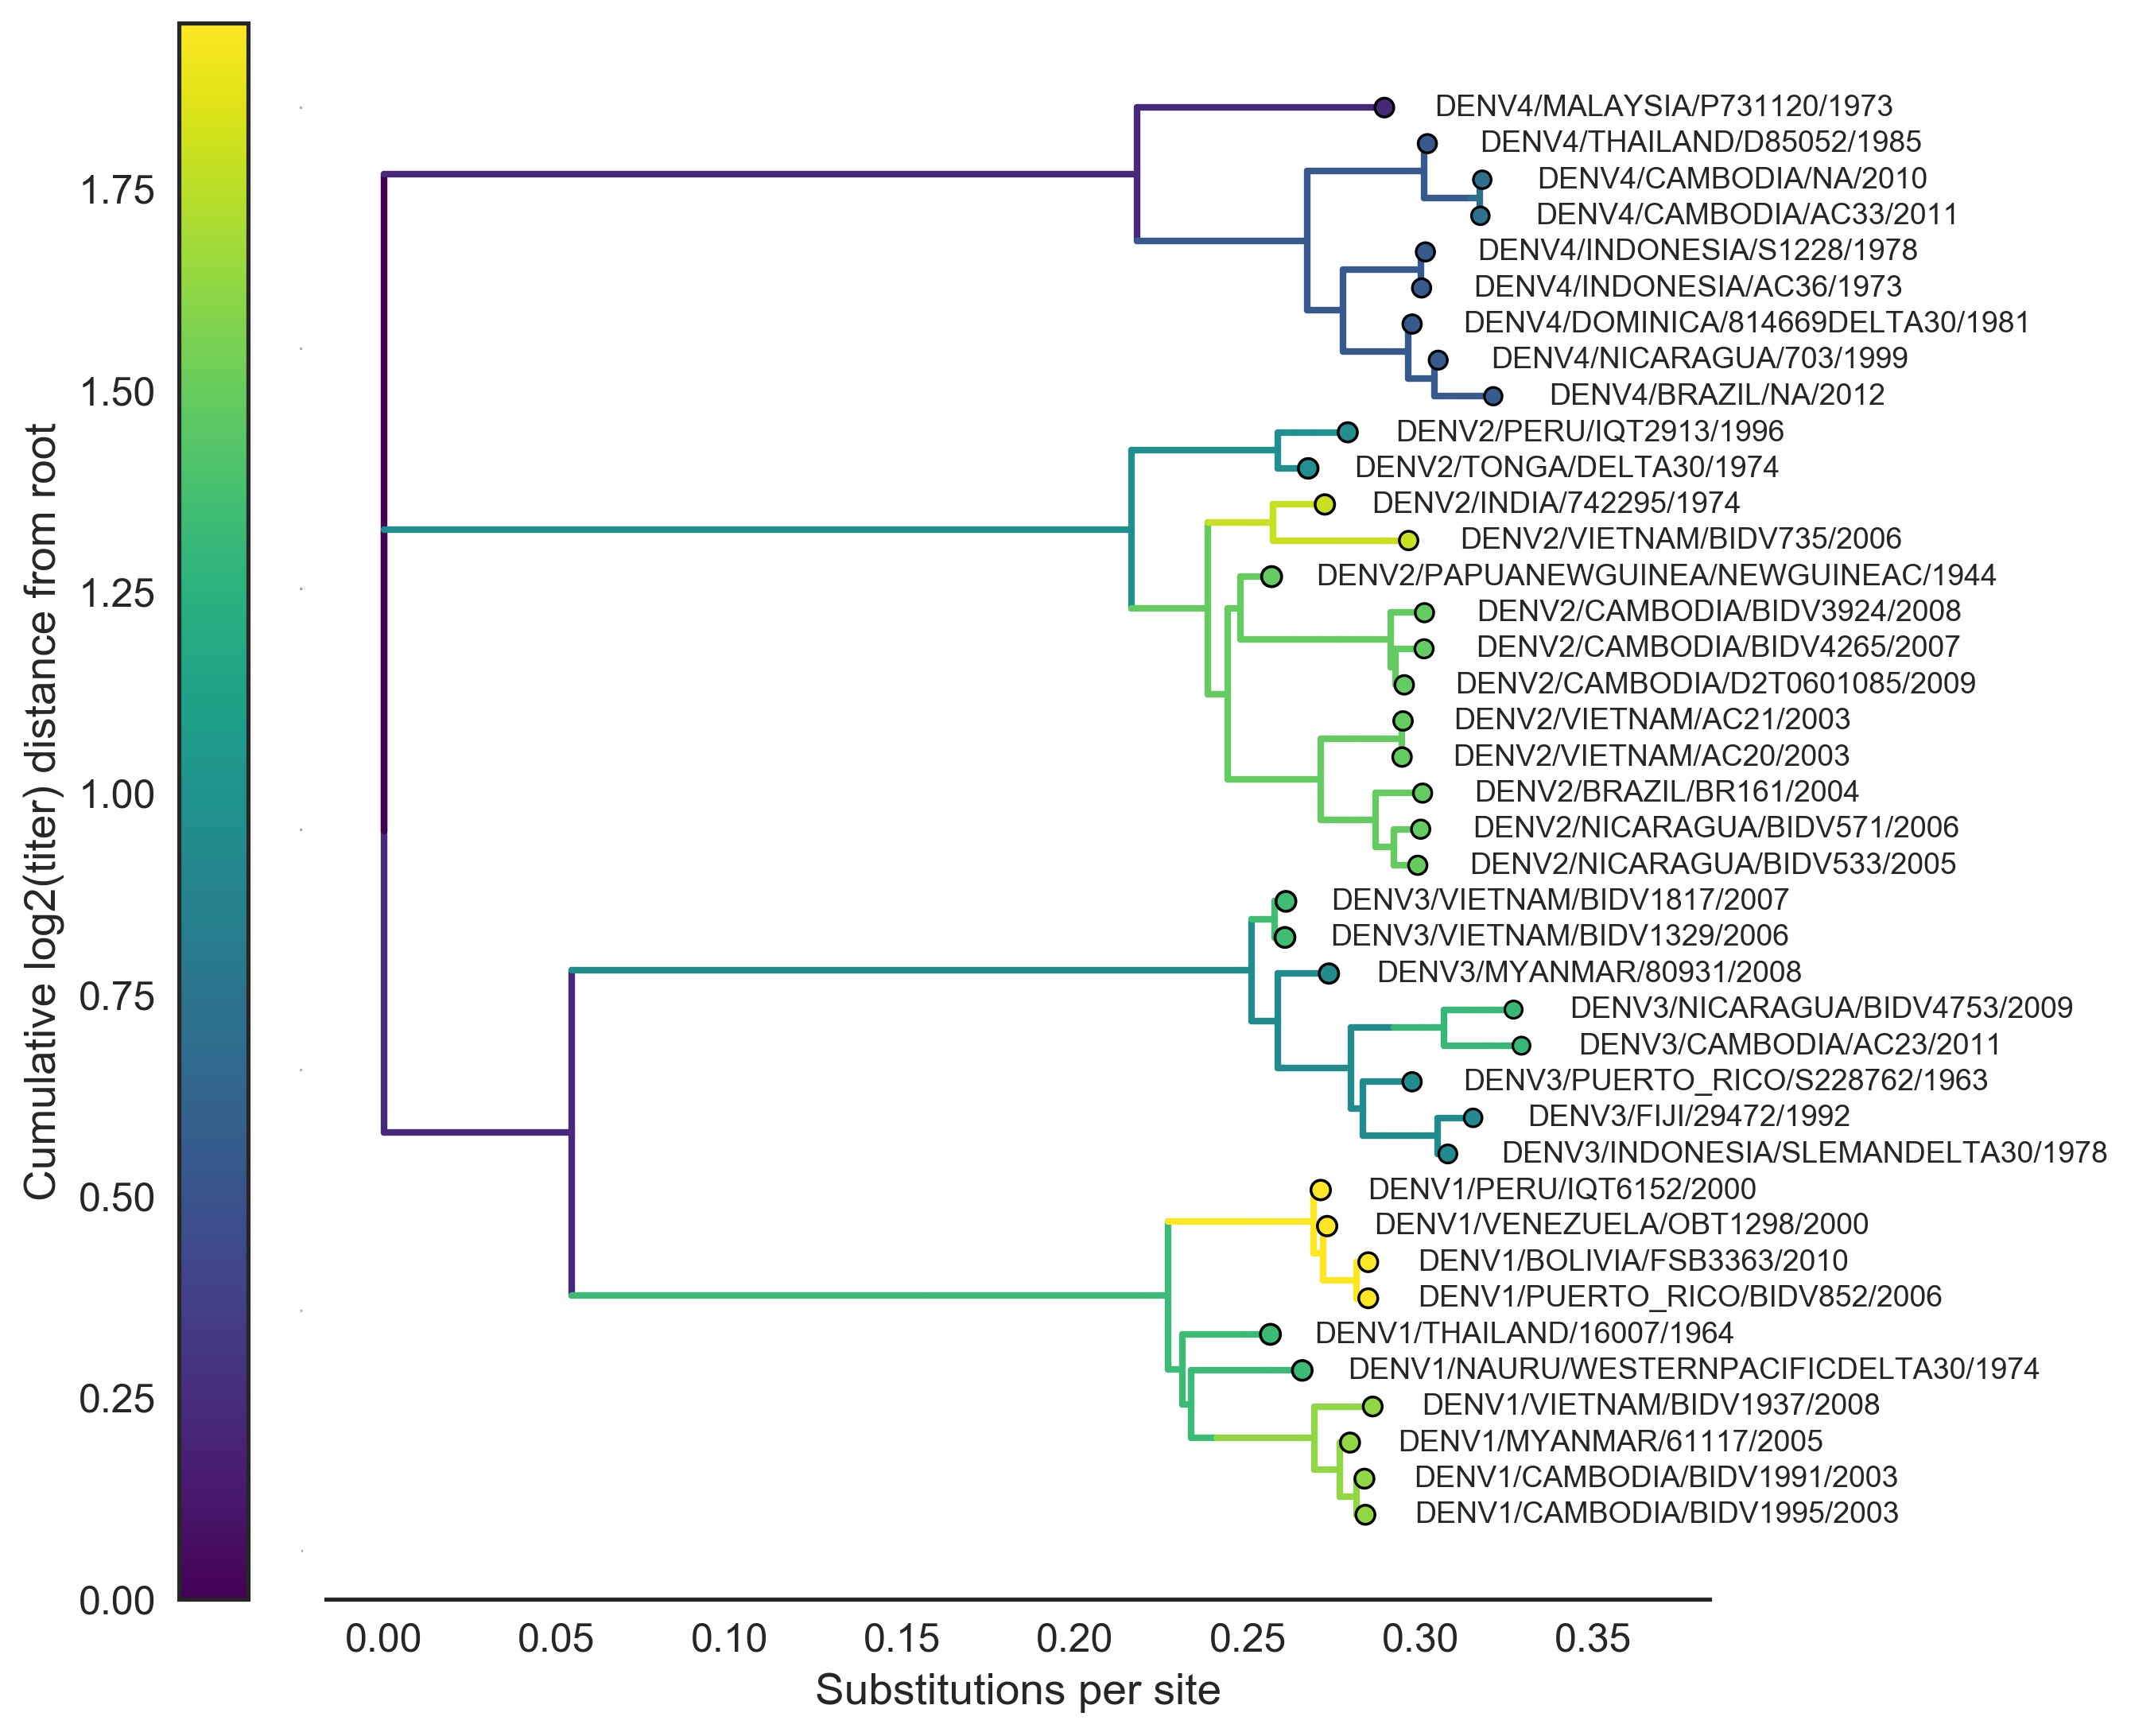
\includegraphics[width=0.65\textwidth]{../figures/png/titered_strains_tree.png}
	\caption{\textbf{Tree of DENV strains in titer dataset}
  Maximum likelihood phylogeny of all DENV strains that were included in the titer dataset. Color represents antigenic divergence from root, as inferred by the `full tree' model.
	}
	\label{titered_strains_tree}
\end{figure}

\begin{figure}[h]
\centering
	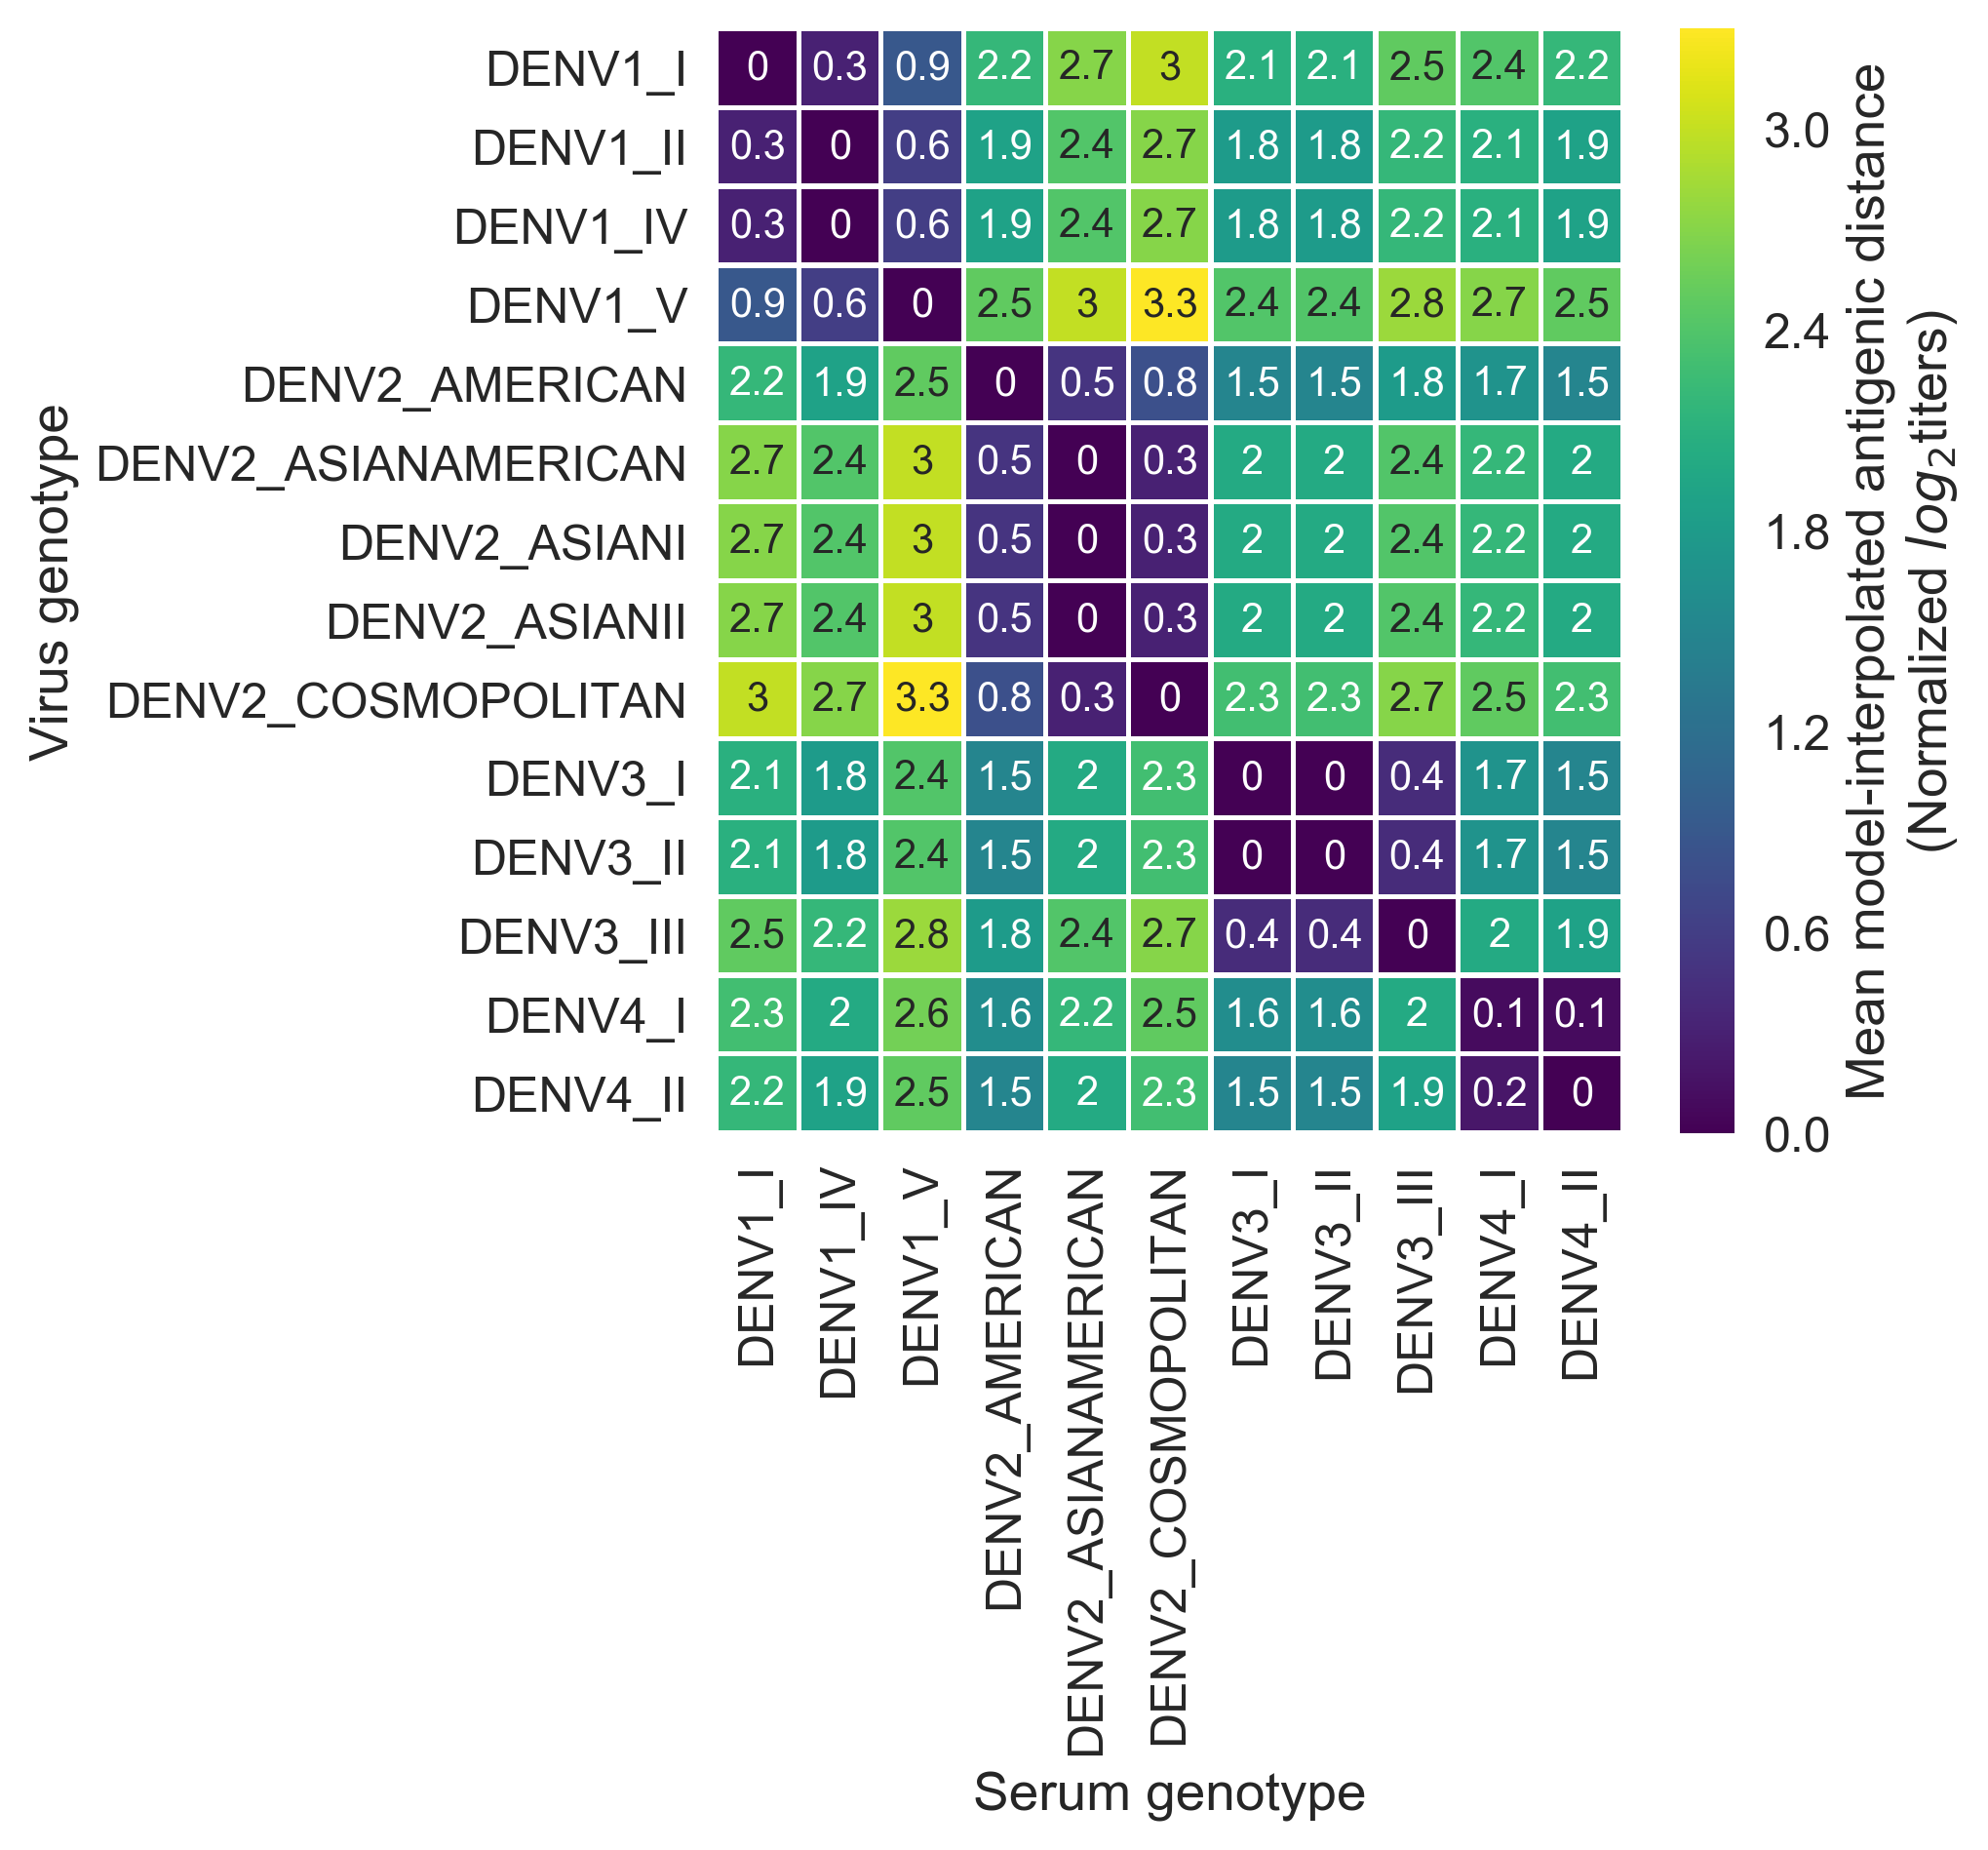
\includegraphics[width=0.65\textwidth]{../figures/png/genotype_dTiter_heatmap.png}
	\caption{\textbf{Titer distance by genotype}
  Values represent the mean antigenic distance between canonical dengue genotypes (in normalized $log_2$ titer units).
  }
	\label{genotype_dTiter_heatmap}
\end{figure}

\begin{figure}[h]
\centering
	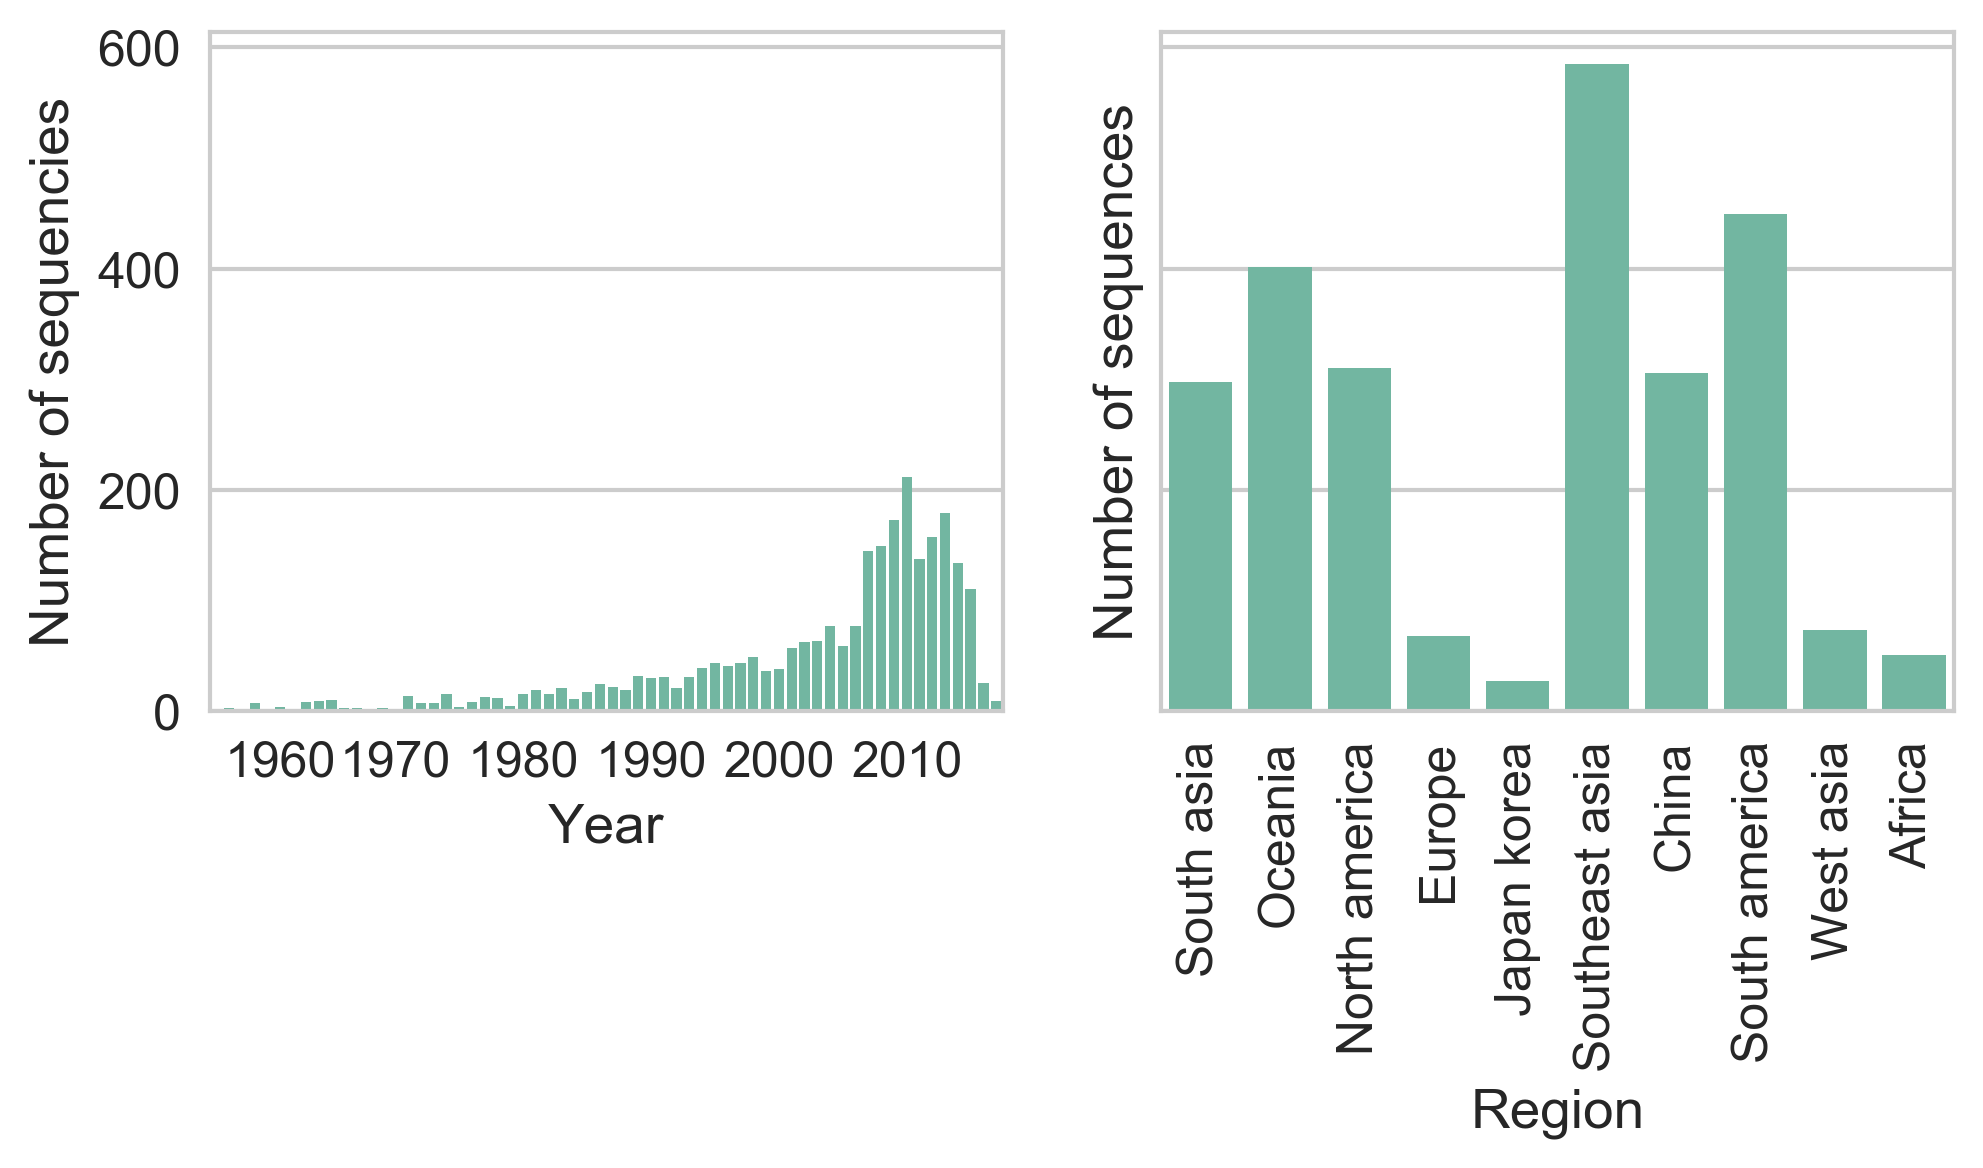
\includegraphics[width=0.65\textwidth]{../figures/png/sequence_distribution.png}
	\caption{\textbf{Sequence dataset distribution}
	}
	\label{sequence_distribution}
\end{figure}


% \begin{figure}[h]
% \centering
% 	\includegraphics[width=0.65\textwidth]{../figures/png/}
% 	\caption{\textbf{SUP FIGURE 1 TITLE }
%
% 	}
% 	\label{SUP_FIGURE_1_LABEL}
% \end{figure}

% \renewcommand{\thetable}{S\arabic{table}}
%
% \begin{longtable}{ | r | l | p{2cm} | l | l | } % COLUMN FORMATS
%
%   \caption{TABLE CAPTION HERE} \label{TABLE LABEL HERE} \\
%   \endfirsthead
%
%   1 & KSA-378 & KJ713296 & camel & 2013-11 \\
%   2 & KSA-363 & KJ713298 & camel & 2013-11 \\
%   3 & KSA-503 & KJ713297 & camel & 2013-11 \\
%
% \end{longtable}

% \begin{figure}[h]
% \centering
% 	% \includegraphics[width=0.65\textwidth]{figures/mers_exploded.png}
% 	\caption{\textbf{SUP FIGURE 1 TITLE }
% SUPP FIGURE 1 CAPTION
% 	}
% 	\label{SUP_FIGURE_1_LABEL}
% \end{figure}


\end{document}
